\documentclass[compress,xcolor=table]{beamer}
\usetheme{Frankfurt}

% Packages
\usepackage[american]{babel}
\usepackage[utf8]{inputenc}
\usepackage[T1]{fontenc}
\usepackage{datetime}
\usepackage{graphicx}
\usepackage{subcaption}
\usepackage{csquotes}
\usepackage{listings}
\usepackage{xcolor}
\usepackage{mathtools}
\usepackage{verbatim}
\usepackage{fancyvrb} % for "\Verb" macro
%\usepackage{transparent}
\usepackage{subfiles} % Best loaded last in the preamble
\usepackage[backend=biber,style=authoryear]{biblatex}
%\usepackage[style=verbose-ibid,backend=bibtex]{biblatex}
%\addbibresource{main.bib}
%\bibliography{main}

%New colors defined below
\definecolor{codegreen}{rgb}{0,0.6,0}
\definecolor{codegray}{rgb}{0.5,0.5,0.5}
\definecolor{codepurple}{rgb}{0.58,0,0.82}
\definecolor{backcolour}{rgb}{0.95,0.95,0.92}
\newcommand{\CoG}{\textcolor{red}}

\newcommand{\pp}{\pause}
%\newcommand{\pp}{~}

%Code listing style named "mystyle"
\lstdefinestyle{mystyle}{
  backgroundcolor=\color{backcolour},   
  commentstyle=\color{codegreen},
  keywordstyle=\color{magenta},
  numberstyle=\tiny\color{codegray},
  stringstyle=\color{codepurple},
  basicstyle=\ttfamily\footnotesize,
  breakatwhitespace=false,         
  breaklines=true,                 
  captionpos=b,                    
  keepspaces=true,                 
  showspaces=false,                
  showstringspaces=false,
  showtabs=false,                  
  tabsize=2
}

\lstset{style=mystyle}

\usepackage{hyperref}
\hypersetup{
    colorlinks=true,
    linkcolor=white,
    filecolor=magenta,      
    urlcolor=cyan,
}

\graphicspath{{images/}}

% Possible options of the package (add/remove below in \usetheme call):
%  - nosectionpages: no pages between sections
%  - flama: use flama font, requires xelatex/lualatex + the font to compile
%  - compressminiframes: put the heading list bullets indications pages on 1 line

\usetheme[compressminiframes]{EuroCC}



% Title page
\title{Introduction to parallel computing in {\tt R}}

%\foottitle{foottitle} % optional, printed at the bottom of the slides, by default same as title, can be useful to rewrite when title has a newline for example
\subtitle{EuroCC training} % optional subtitle
\date{\formatdate{18}{1}{2024}}
\author{prof. dr. Janez Povh \\ dr. Tomas Martinović (Rcpp)}

\institute{University of Ljubljana} 
\institute{EuroHPC Competence Center, October 25, \monthyeardate{2024}}
% Optional

% Biblatex
% \usepackage[backend=biber, style=apa]{biblatex}
% \bibliography{library.bib}
% \renewcommand*{\bibfont}{\footnotesize}

%%%%
%% BEGIN OF SLIDES
%%%%

\begin{document}

% \nocite{*}

{\usebackgroundtemplate{%
  \includegraphics[width=\paperwidth,height=\paperheight]{"EuroCC Background DARK_rectangular.png"}} 
\begin{frame}[plain]
\titlepage
\setcounter{framenumber}{0}
\end{frame}
}

%{
%\setcounter{tocdepth}{1}
%\setbeamertemplate{section in toc}[ball unnumbered]
%{\setbeamercolor{background canvas}{bg=EuroCCBeige}
%\begin{frame}[plain]
%\frametitle{Outline}
%\tableofcontents
%\end{frame}}
%}

%\begingroup
%    \AtBeginSection[]{}
%\section{Schedule} 
%\subfile{sections/00_schedule}

%\endgroup


\section{Introduction to HPC} 




\begin{frame}{What is HPC}
\begin{figure}
				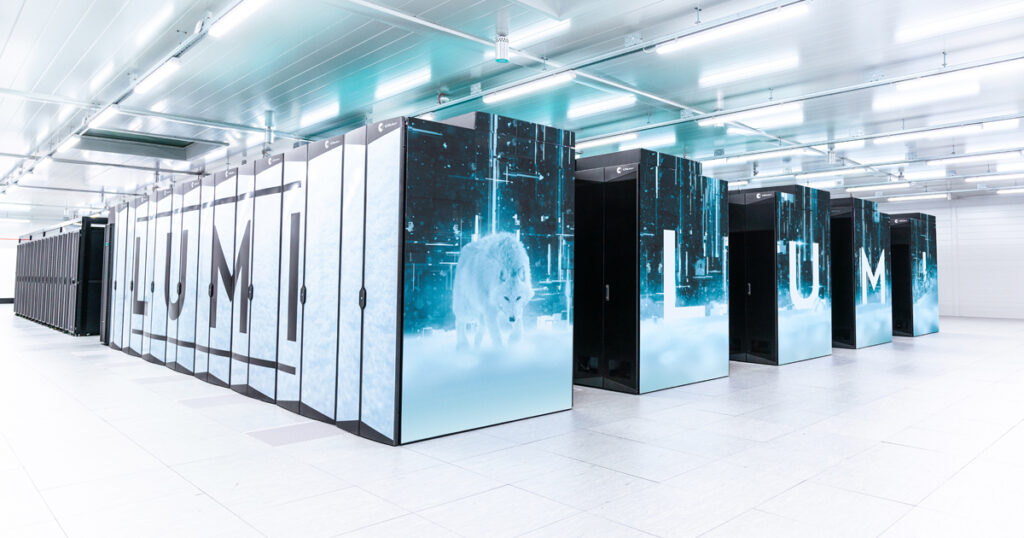
\includegraphics[width=200pt]{images/LUMI2.jpg}

\scriptsize Source: https://www.vyzkumne-infrastruktury.cz/en/2022/06/lumi-supercomputer-has-been-inaugurated/
\end{figure}

\end{frame}	




\begin{frame}{What is HPC}
	\begin{figure}
	\begin{center}
	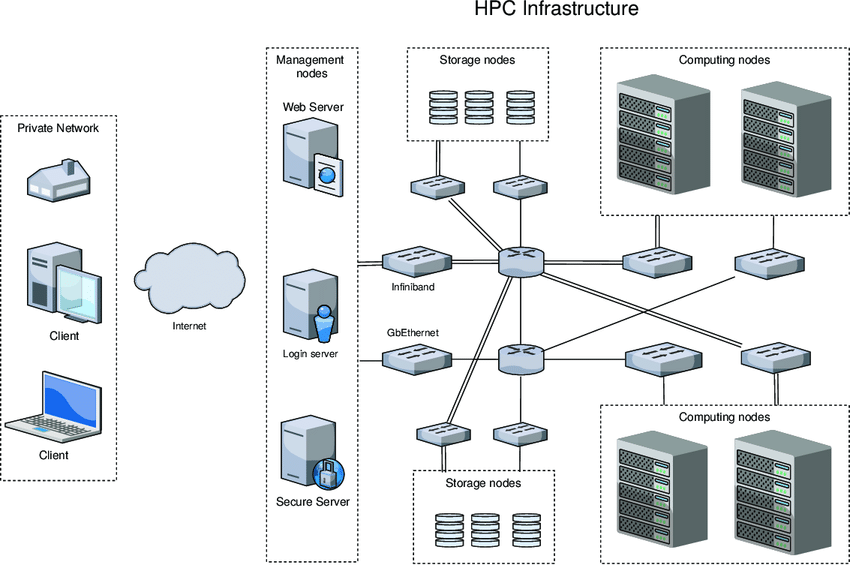
\includegraphics[width=0.6\textwidth]{images/HPC_structure}
	
	Source: Reghenzani, F. et al,  IEEE Access, 8, 208566-208582.

    \end{center}

	\end{figure}
\end{frame}	


\begin{frame}{Node structure}
	\begin{center}
		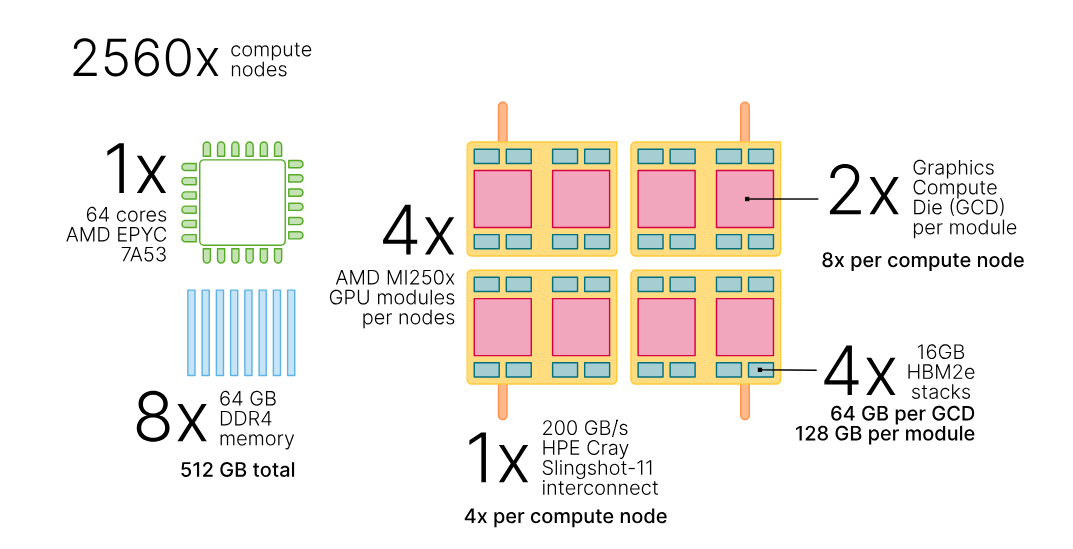
\includegraphics[width=0.6\textwidth]{images/Node_Lumi}
		
		Source: https://docs.lumi-supercomputer.eu/hardware/lumig/
	\end{center}
\end{frame}


\begin{frame}{How does my computer look like}
	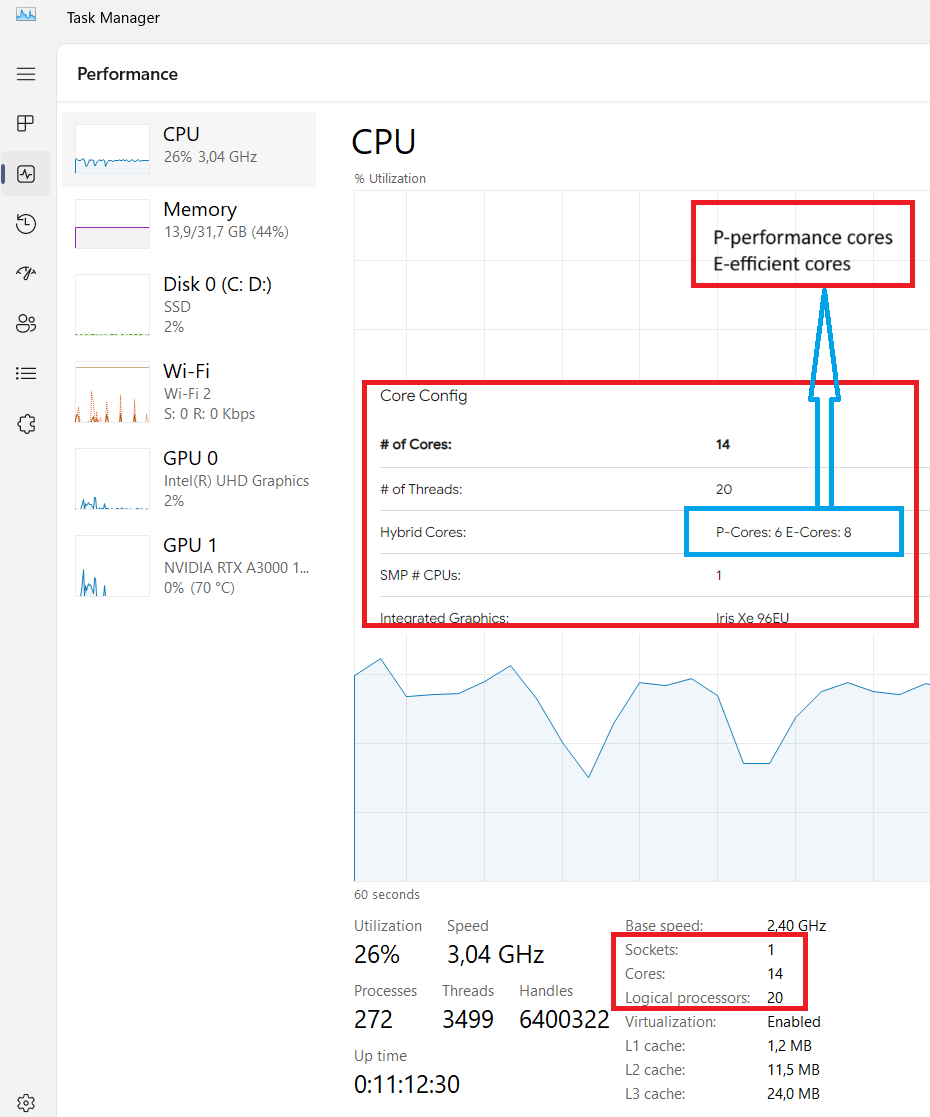
\includegraphics[width=150pt]{images/windows_task_manager.png}
\end{frame}


\begin{frame}{How does my computer looks like}
	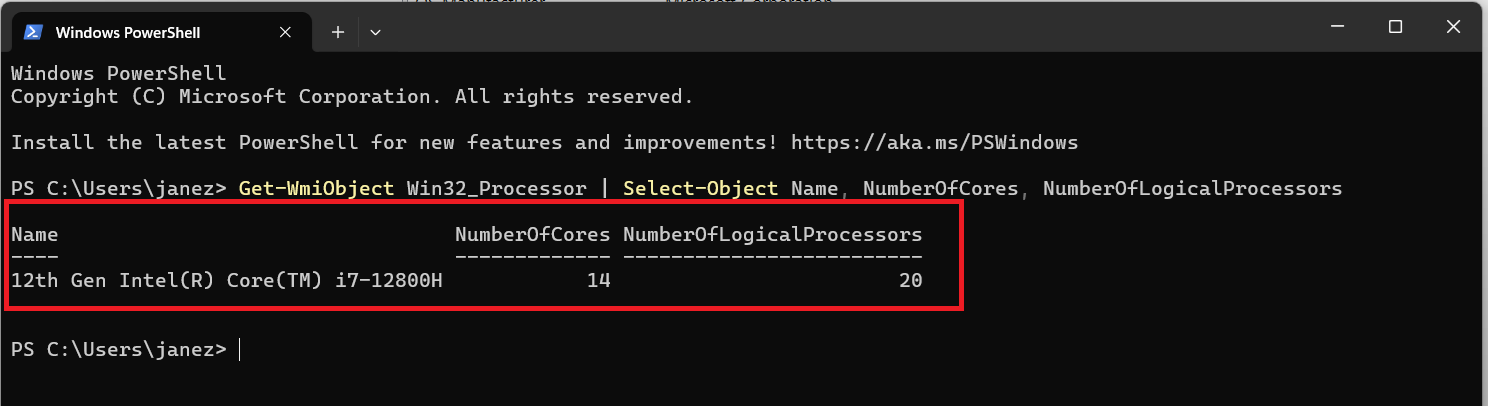
\includegraphics[width=250pt]{images/power_shell.png}
\end{frame}

\begin{comment}
	
\begin{frame}{How does Barbora cluster look like}
	192 standard computing nodes (2x18 cores), 8 GPU nodes, 1 fat node (6TB RAM)
	
	
\includegraphics[width=250pt]{images/barbora.jpg}
\end{frame}

\end{comment}


\begin{frame}{Why HPC}
	Some computations are (very) extensive:
	\begin{itemize}
		\item \CoG{cpu-extensive:} take too much cpu time\pp 
		\item \CoG{memory-extensive:} Take too much memory\pp 
		\item \CoG{I/O-extensive:} Take too much time to read/write from disk\pp 
		\item \CoG{network-extensive:} Take too much time to transfer over the network.
	\end{itemize}
\end{frame}


\begin{frame}{User experience}
	\begin{center}
		
		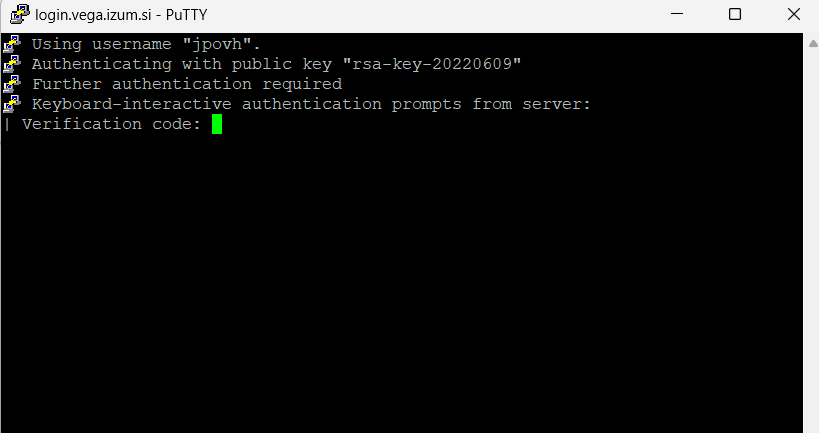
\includegraphics[width=0.8\textwidth]{images/ssh.png}
		
	\end{center}
\end{frame}

\begin{frame}{How to access HPC}
	HPCs are \textcolor{red}{easily} available. 
	\begin{center}
		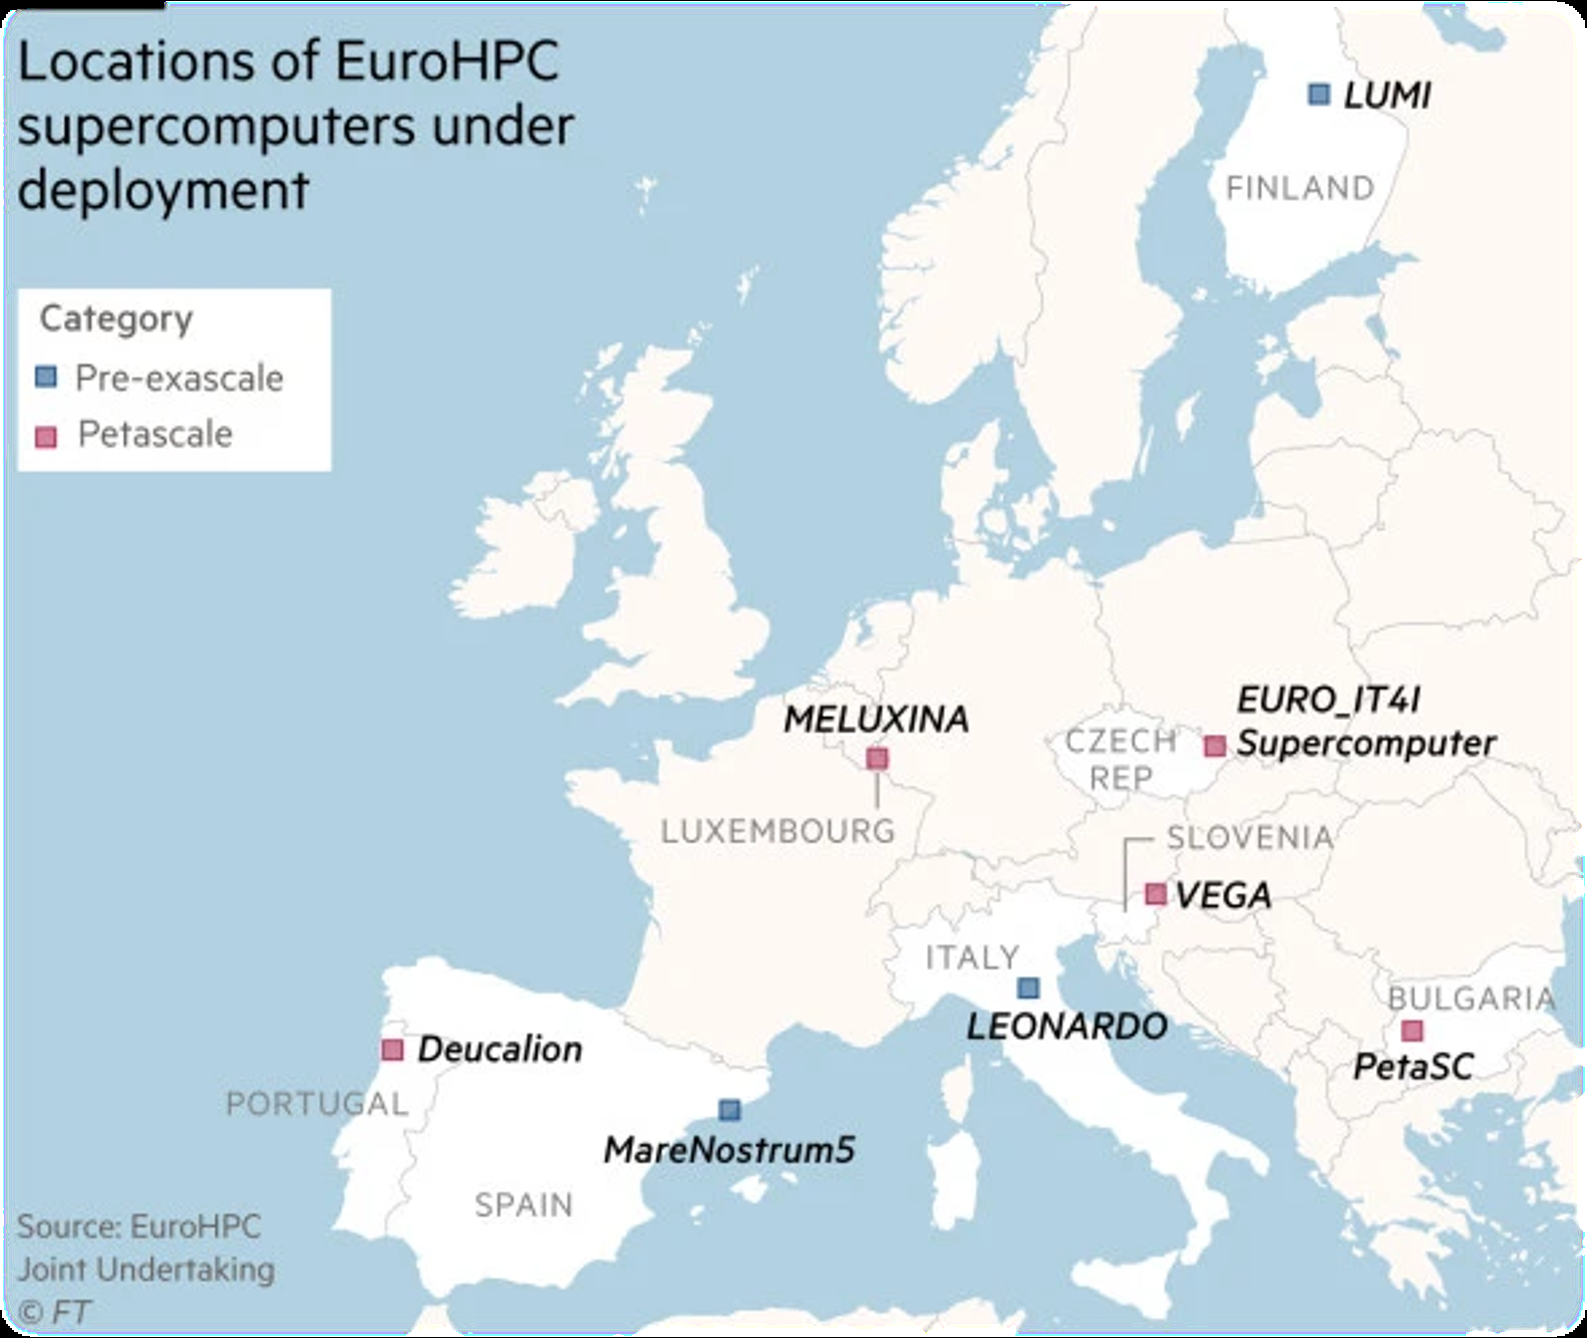
\includegraphics[width=220pt]{images/HPCmap}
		
	\end{center}
	
\end{frame}

\begin{frame}{EuroCC2}
	\begin{itemize}
		\item Network of EU Competence centers for HPC.\pp
		\item All members of EuroHPC JU involved.\pp
		\item Training, support for industry, talent attraction,...
	\end{itemize}
\end{frame}




\section{Introduction to R} 
\subsection{Basics about R}

\begin{frame}{What is R}
	\begin{itemize}
		\item Software for Statistical Data Analysis
		\item  Based on S
		\item Cores routines are written and Fortran
		\item  Programming Environment
		\item  Interpreted Language
		\item  Data Storage, Analysis, Visualization
		\item  Free and Open Source Software
	\end{itemize}
\end{frame}

\begin{frame}{How to obtain R}
	\begin{itemize}
		\item R current version 4.4.1 (released June 2024).
		\item \url{http://cran.r-project.org}
		\item Binary/Windows executable code
	\end{itemize}
\end{frame}


\begin{frame}{Pros and Cons}
	Pros:
	\begin{itemize}
		\item 	Free and Open Source
		\item Strong User Community
		\item Highly extensible, flexible
		\item Implementation of high-end statistical methods
		\item Flexible graphics and intelligent defaults
	\end{itemize}\pp 
	
	Cons
	\begin{itemize}
		\item Steep learning curve
		\item Slow for large datasets
	\end{itemize}
	
\end{frame}




\begin{frame}{Data types}
	\begin{itemize}
		\item R Supports virtually any type of data
		\item 	Numbers, characters, logicals (TRUE/ FALSE)
		\item 	Arrays of virtually unlimited sizes
		\item 	Simplest: Vectors and Matrices
		\item 	Lists: Can Contain mixed type variables
		\item 	Data Frame: Rectangular Data Set
		\item  Datasets in {\tt tidy} format.
		
	\end{itemize}
\end{frame}




\begin{frame}{Data structures in R}
	Linear
	\begin{itemize}
		\item vectors (all same type)
		\item lists (mixed types)
	\end{itemize}\pp 
	Rectangular
	\begin{itemize}
		\item data frame
		\item matrix
	\end{itemize}
	
\end{frame}

%\subsection{Running R}

\begin{frame}{Running R}
	\begin{itemize}
		\item I recommend RStudio, an IDE for R.\pp 
		\item It is available as RStudio Desktop and \textbf{RStudio Server}, which runs on a remote server and allows accessing RStudio using a web browser.
		
	\end{itemize}
	
	
	
	\begin{figure}
		\includegraphics[width=180pt]{images/rstudio1} 
		\caption{\scriptsize \url{https://rstudio.com/products/rstudio/download/}}
	\end{figure}
\end{frame}


\begin{comment}
	

\begin{frame}{RStudio on IT4I}
	
	\begin{itemize}
		\item Run RStudio on VM.\pp 
		\item \small Connect to \url{shiny.vsb.cz/auth}  \pp
		 
	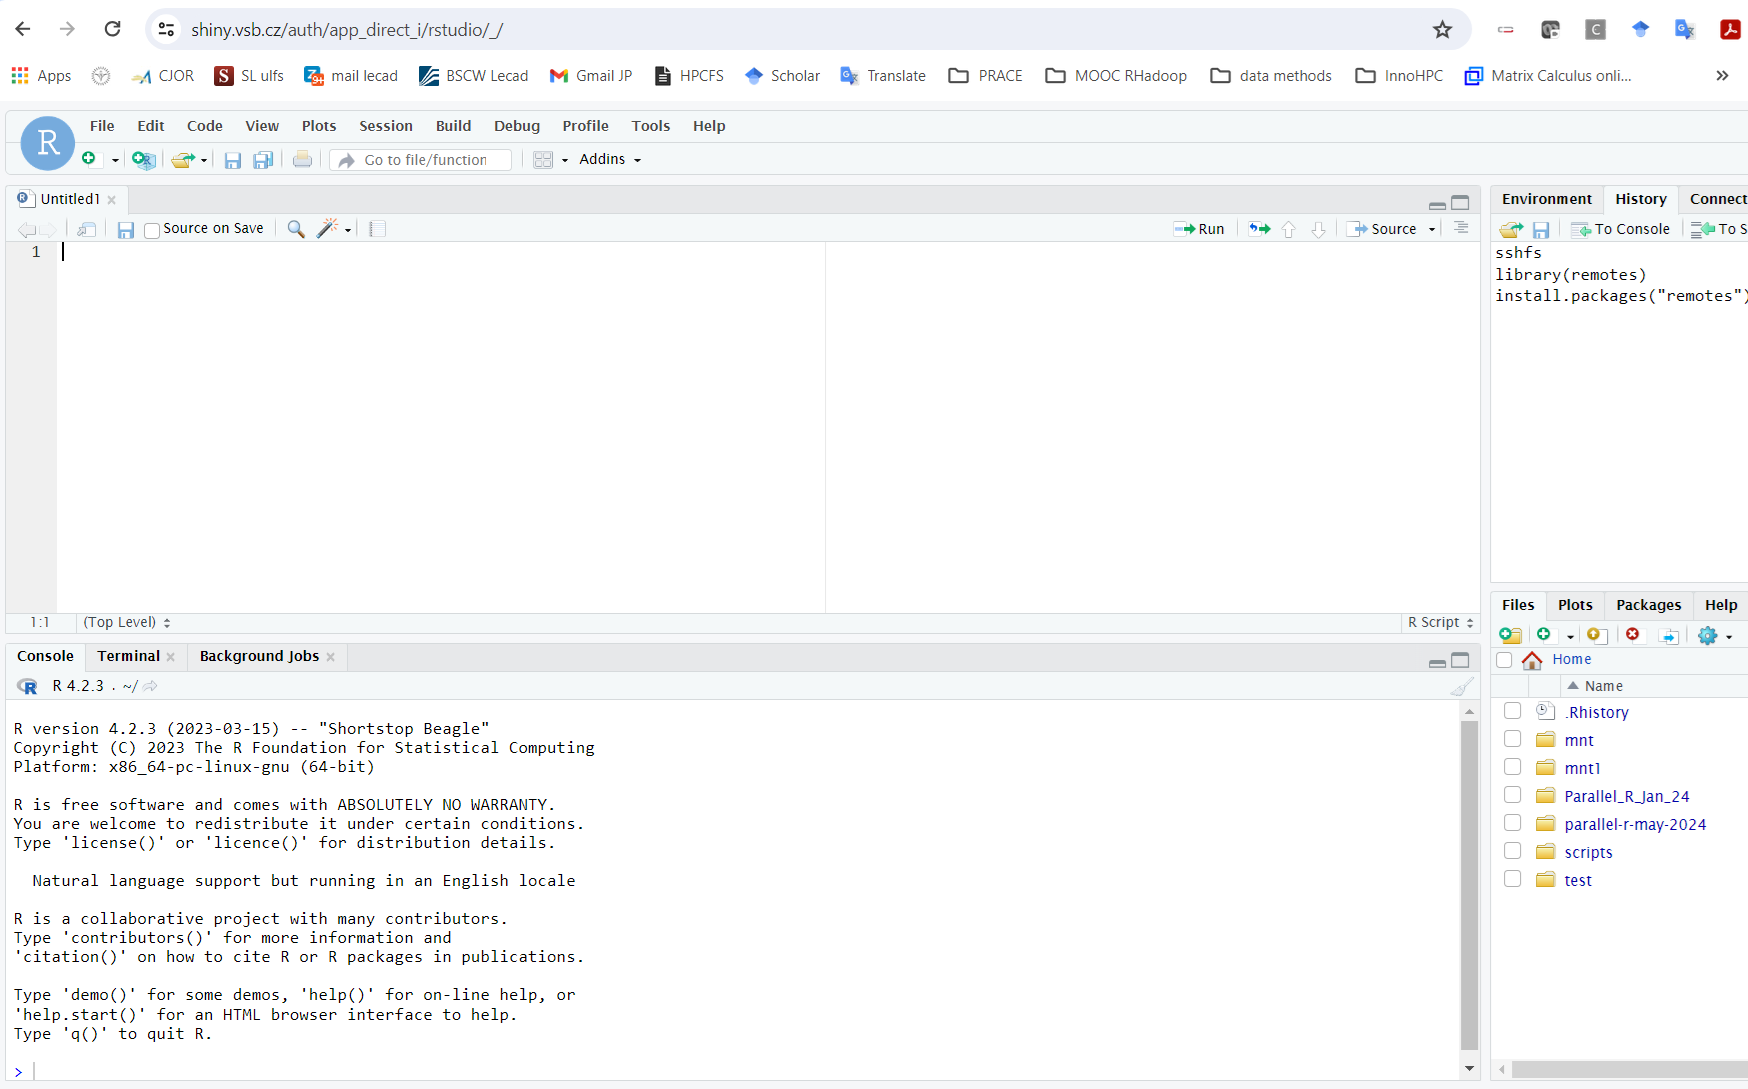
\includegraphics[width=250pt]{images/shiny} 
	
	\end{itemize}
\end{frame}


\end{comment}

\begin{frame}{Clone the data}
	
		Clone project from GITHUB \url{https://github.com/janezpovh/parallel-R-sep-24}
		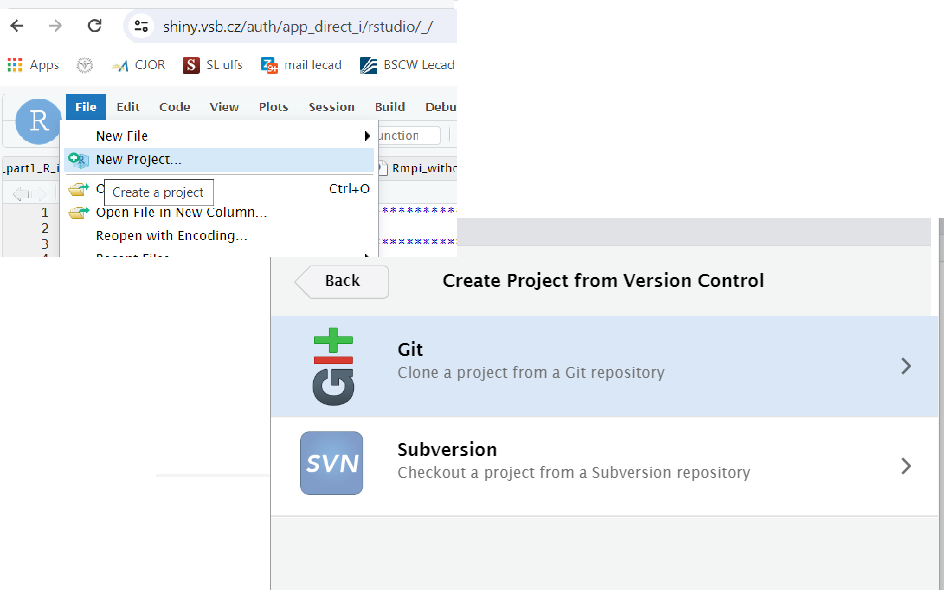
\includegraphics[width=180pt]{images/git1} 
		
\end{frame}

\begin{comment}

\begin{frame}{Connect to HPC using NoMachine}
	Main steps
	\begin{itemize}
		\item Connect to HPCFS to gpu02 login node
		\item Rund Rstudio on login node OR
		\item Connect to compute node and run Rstudio on compute node. 
	\end{itemize}
\end{frame}


\subsection{Connect to HPCFS}

\begin{frame}{Download Nomachine Enterprise Client}
	
	
\includegraphics[width=240pt]{images/Nomachine1.png} 	
	
\end{frame}	



\begin{frame}{Install Nomachine Client}
	
	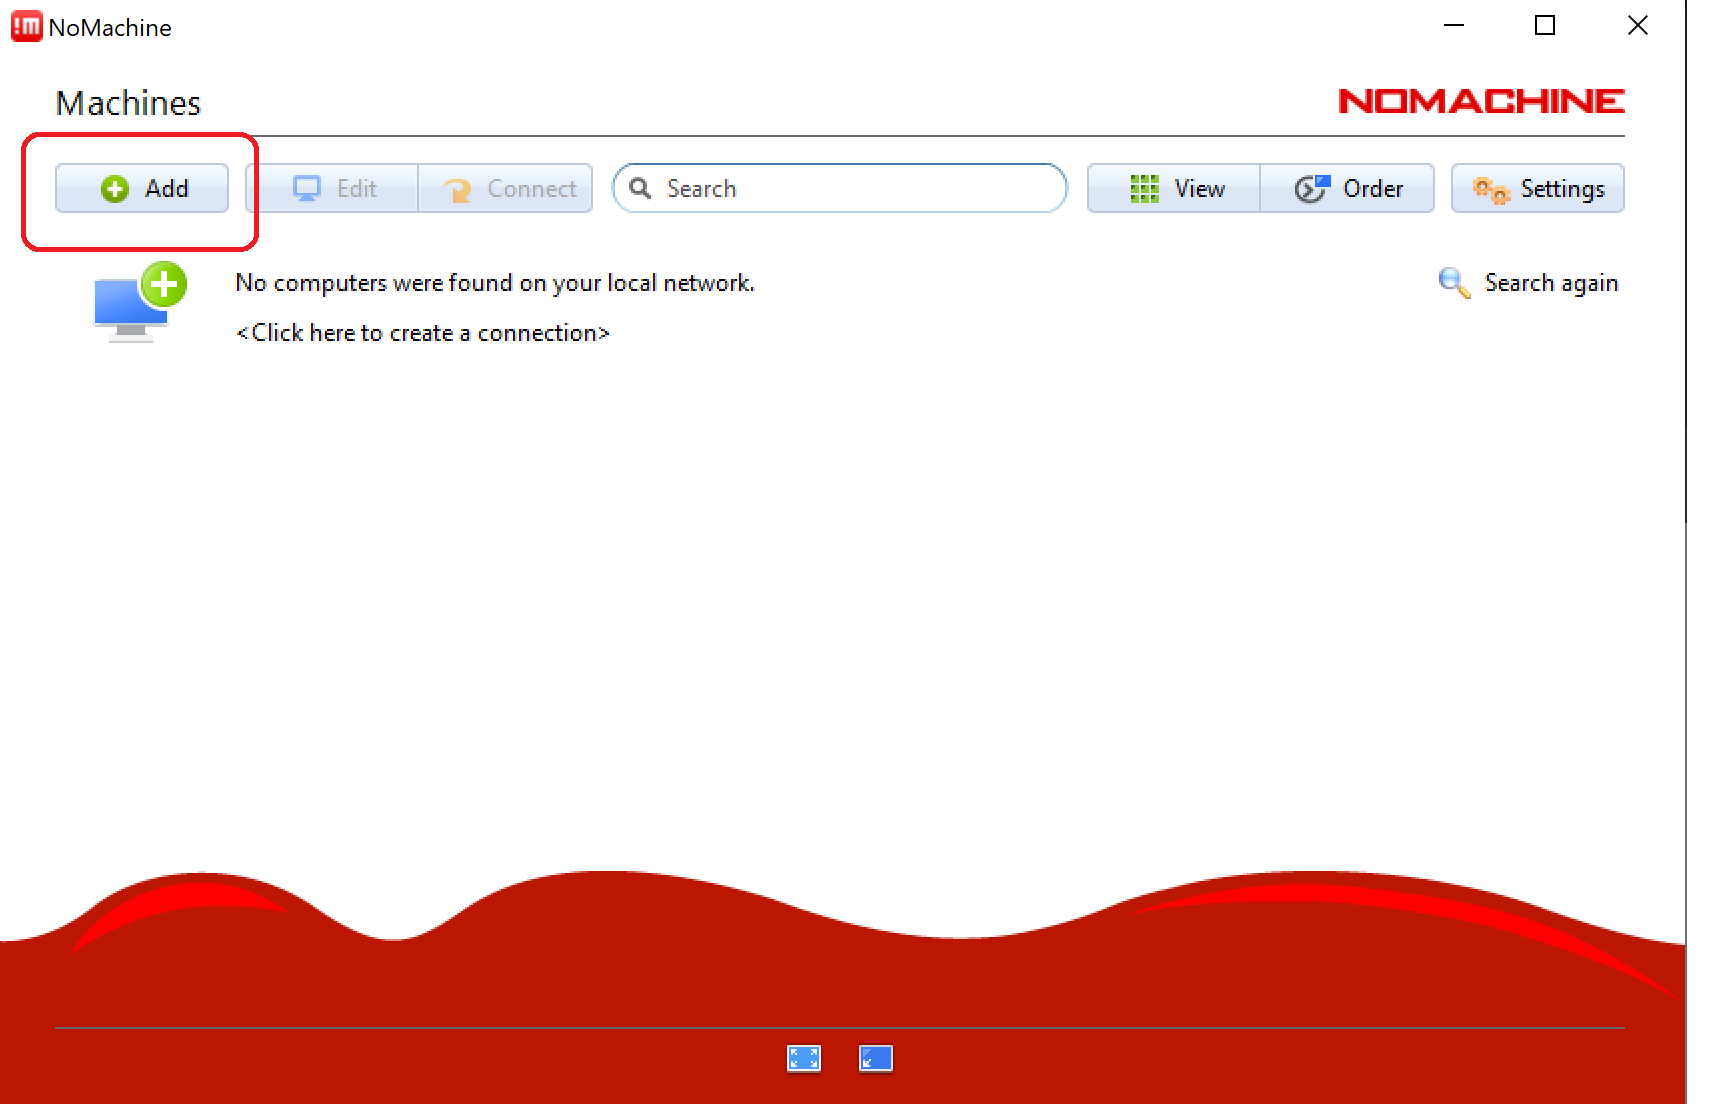
\includegraphics[width=240pt]{images/slika1} 	
	
\end{frame}	




\begin{frame}{Enter data for HPCFS}
	
	HOST: login.hpc.fs.uni-lj.si
	Name: whatever you want
	
	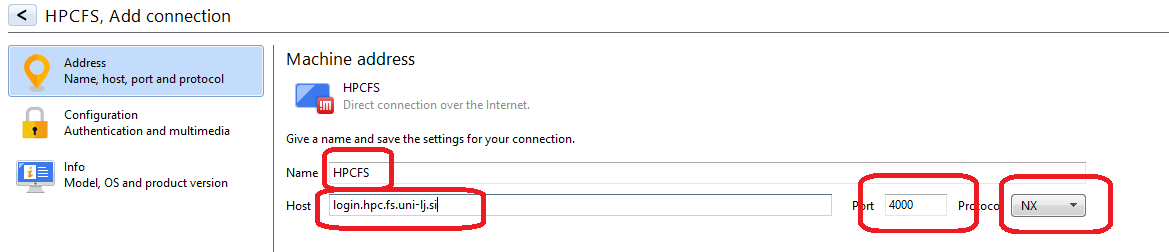
\includegraphics[width=240pt]{images/slika8} 	
	
\end{frame}	

\begin{frame}
	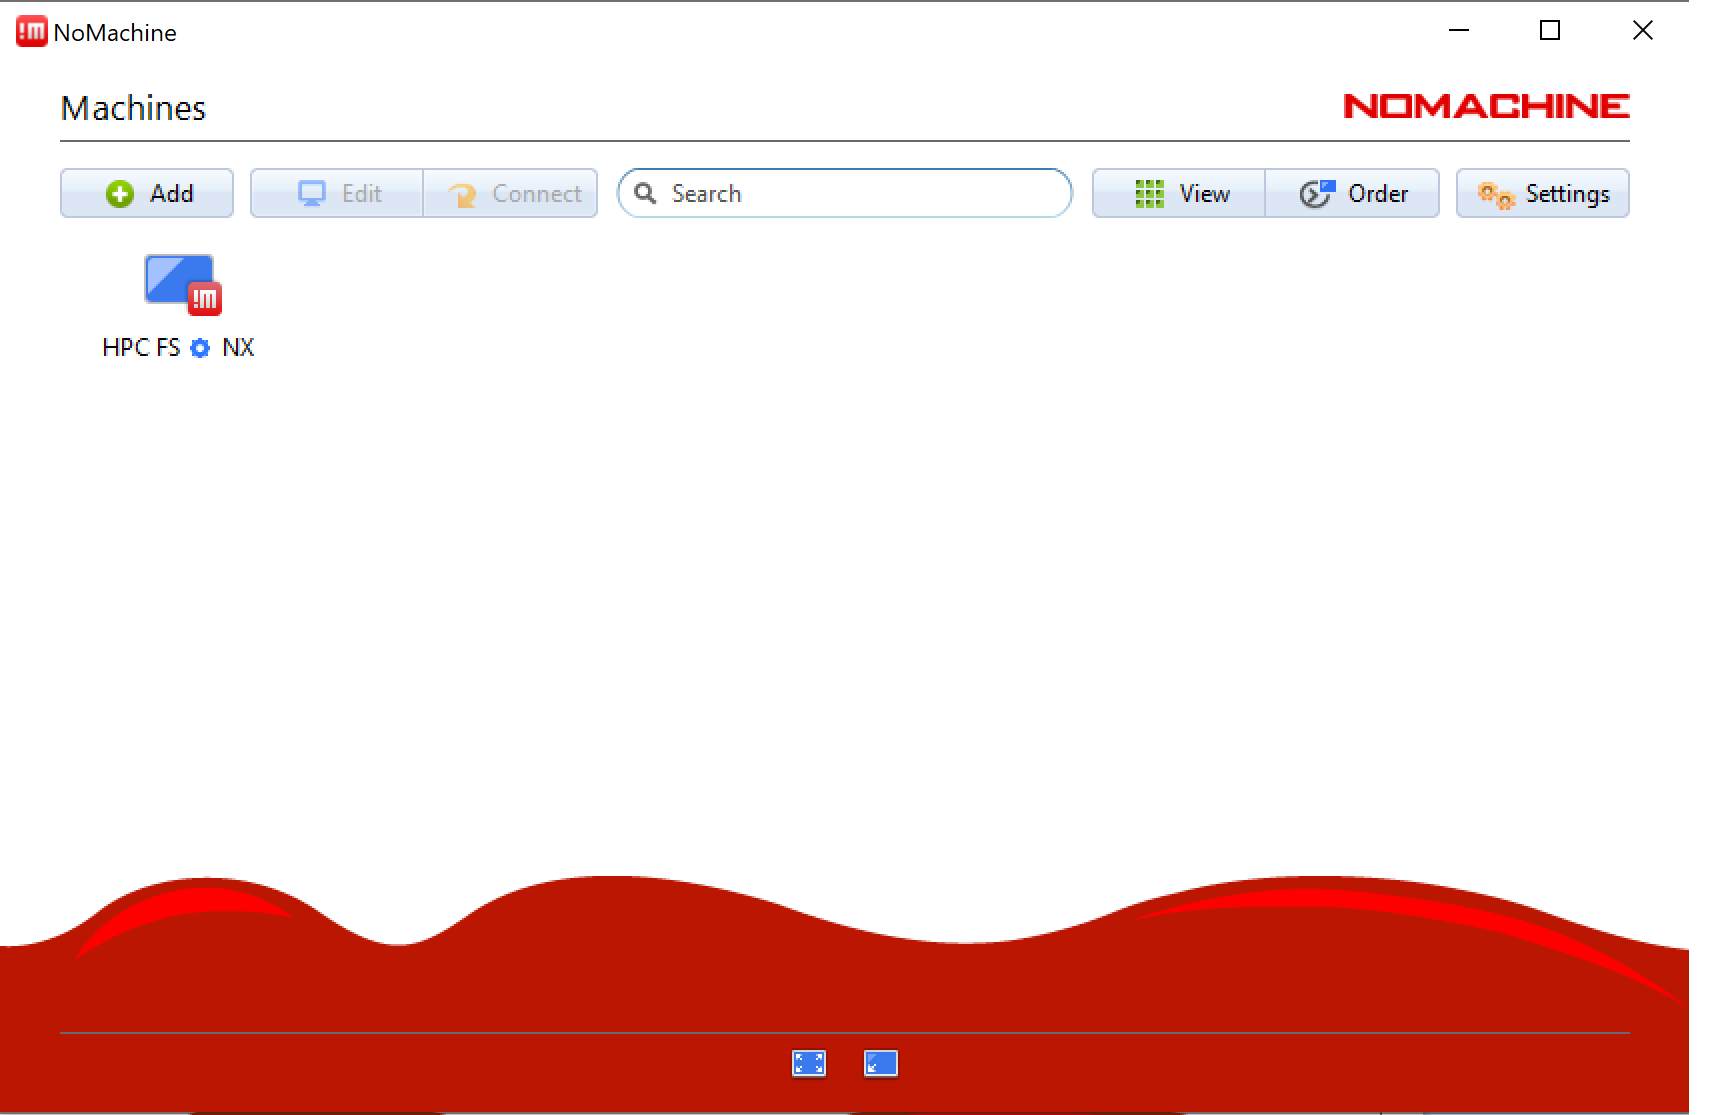
\includegraphics[width=240pt]{images/slika2} 	
	
\end{frame}	



\begin{frame}{Skip autentification warning}
	
	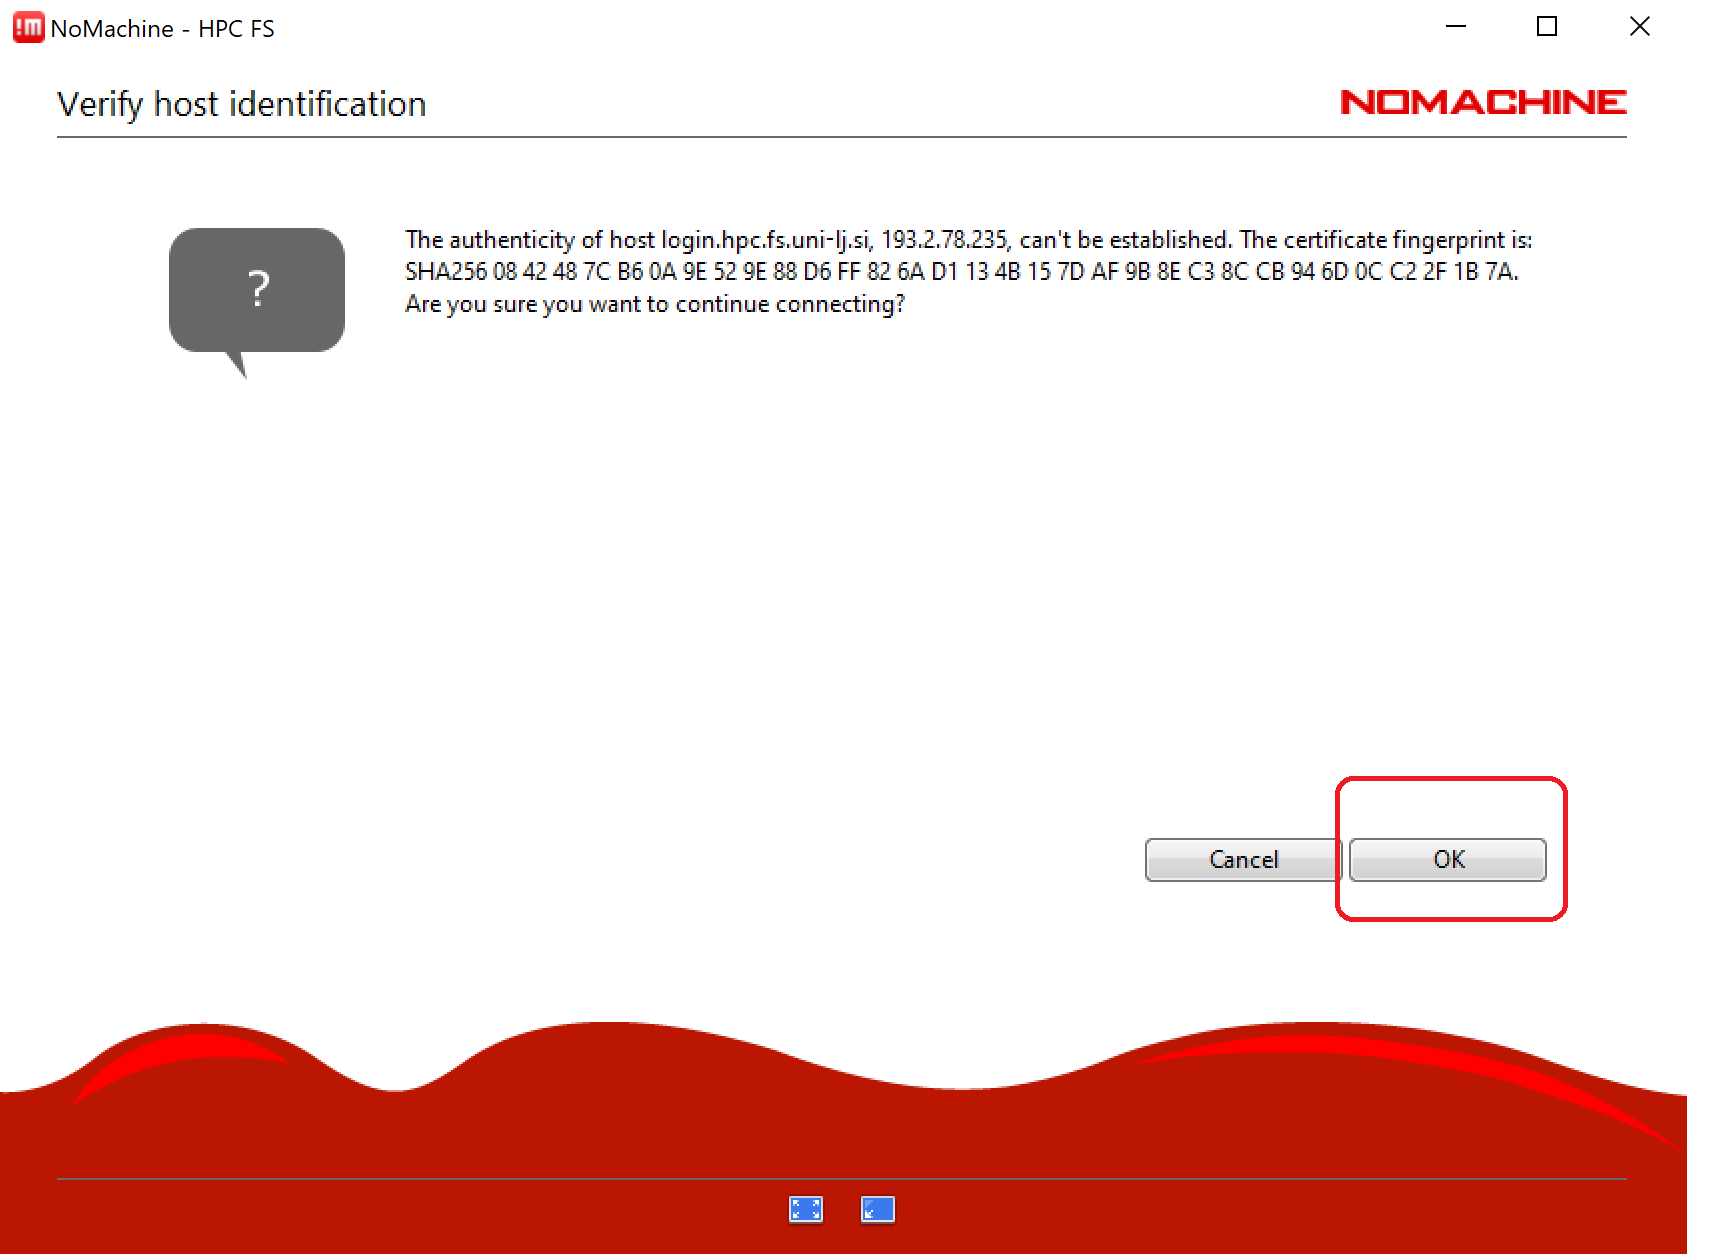
\includegraphics[width=240pt]{images/slika3} 	
	
\end{frame}	


\begin{frame}{Enter credentials}
	
	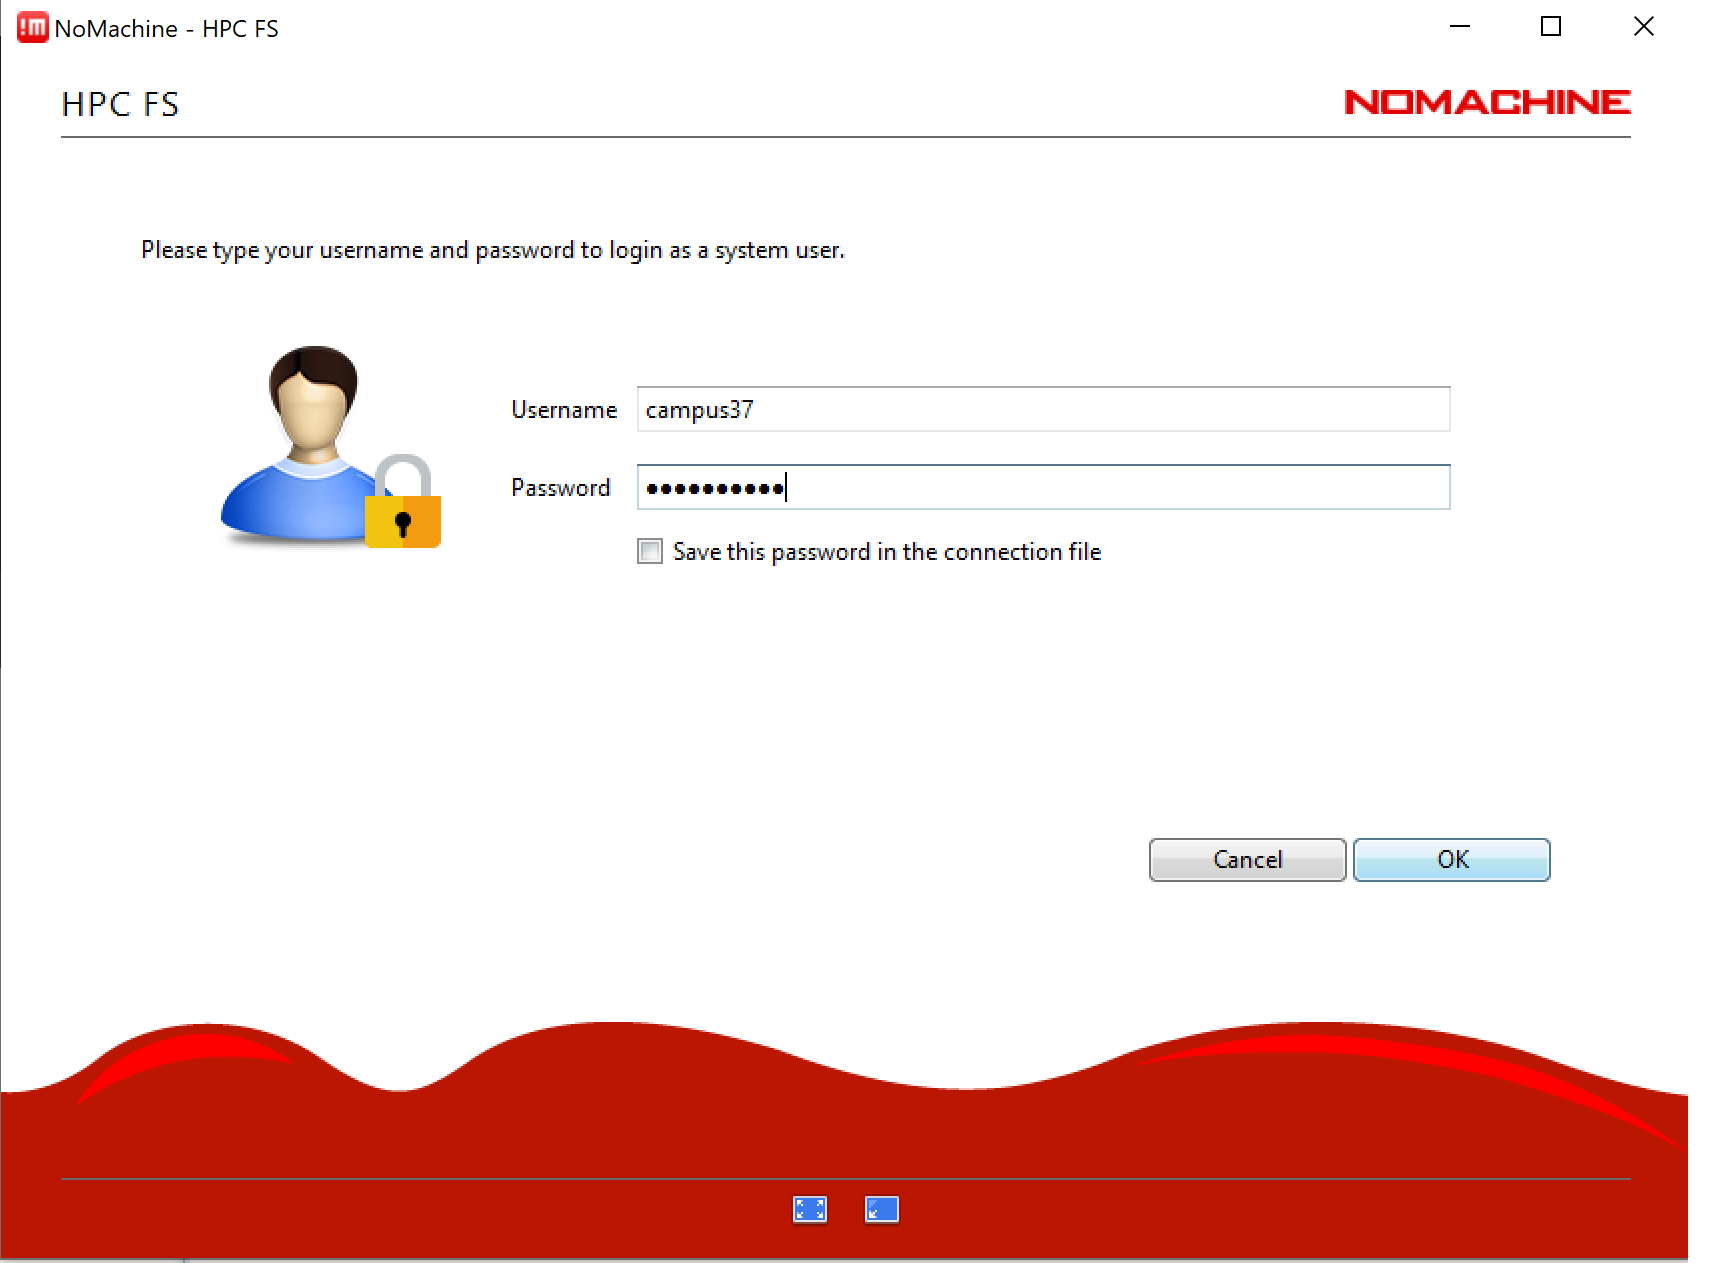
\includegraphics[width=240pt]{images/slika4} 	
	
\end{frame}	



\begin{frame}{Create new virtual desktop}
	
	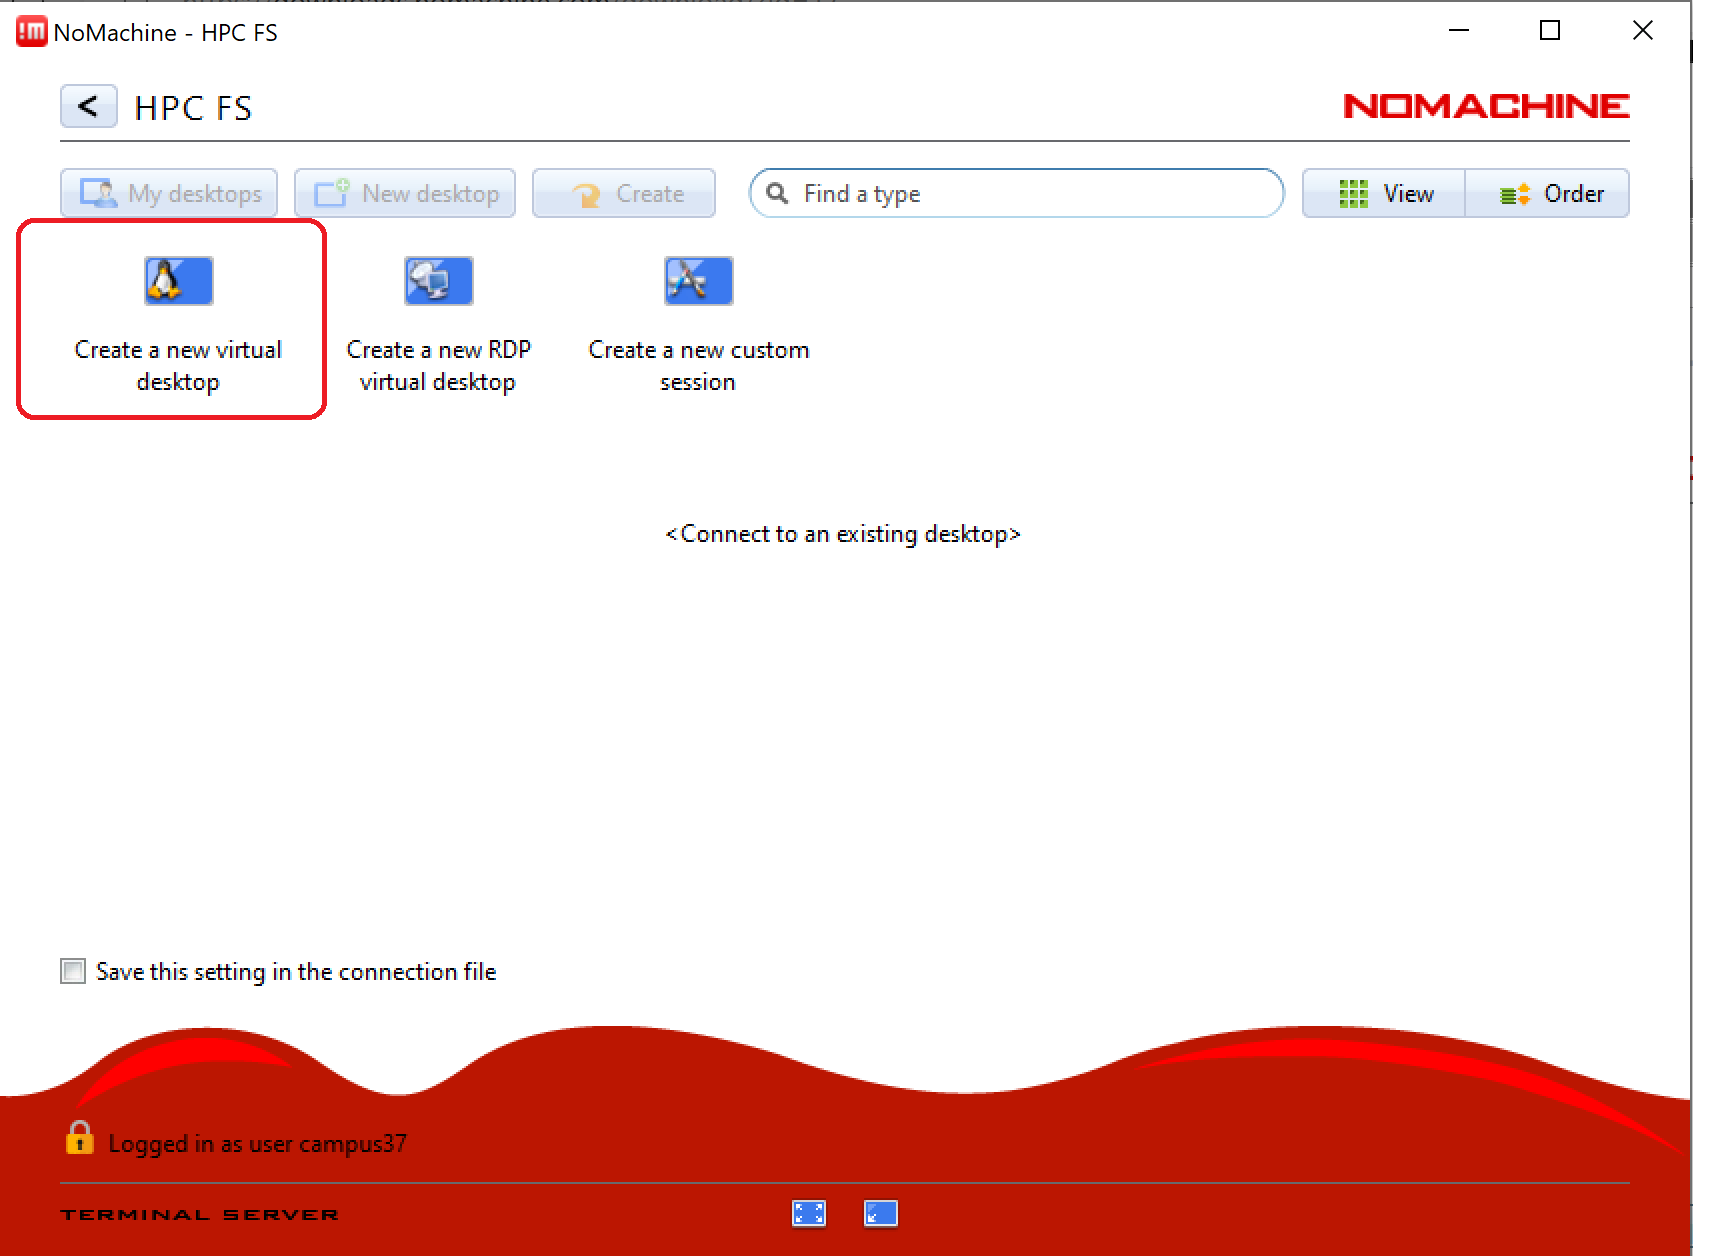
\includegraphics[width=240pt]{images/slika5} 	
	
\end{frame}	




\begin{frame}{Define remote desktop setting}
	
	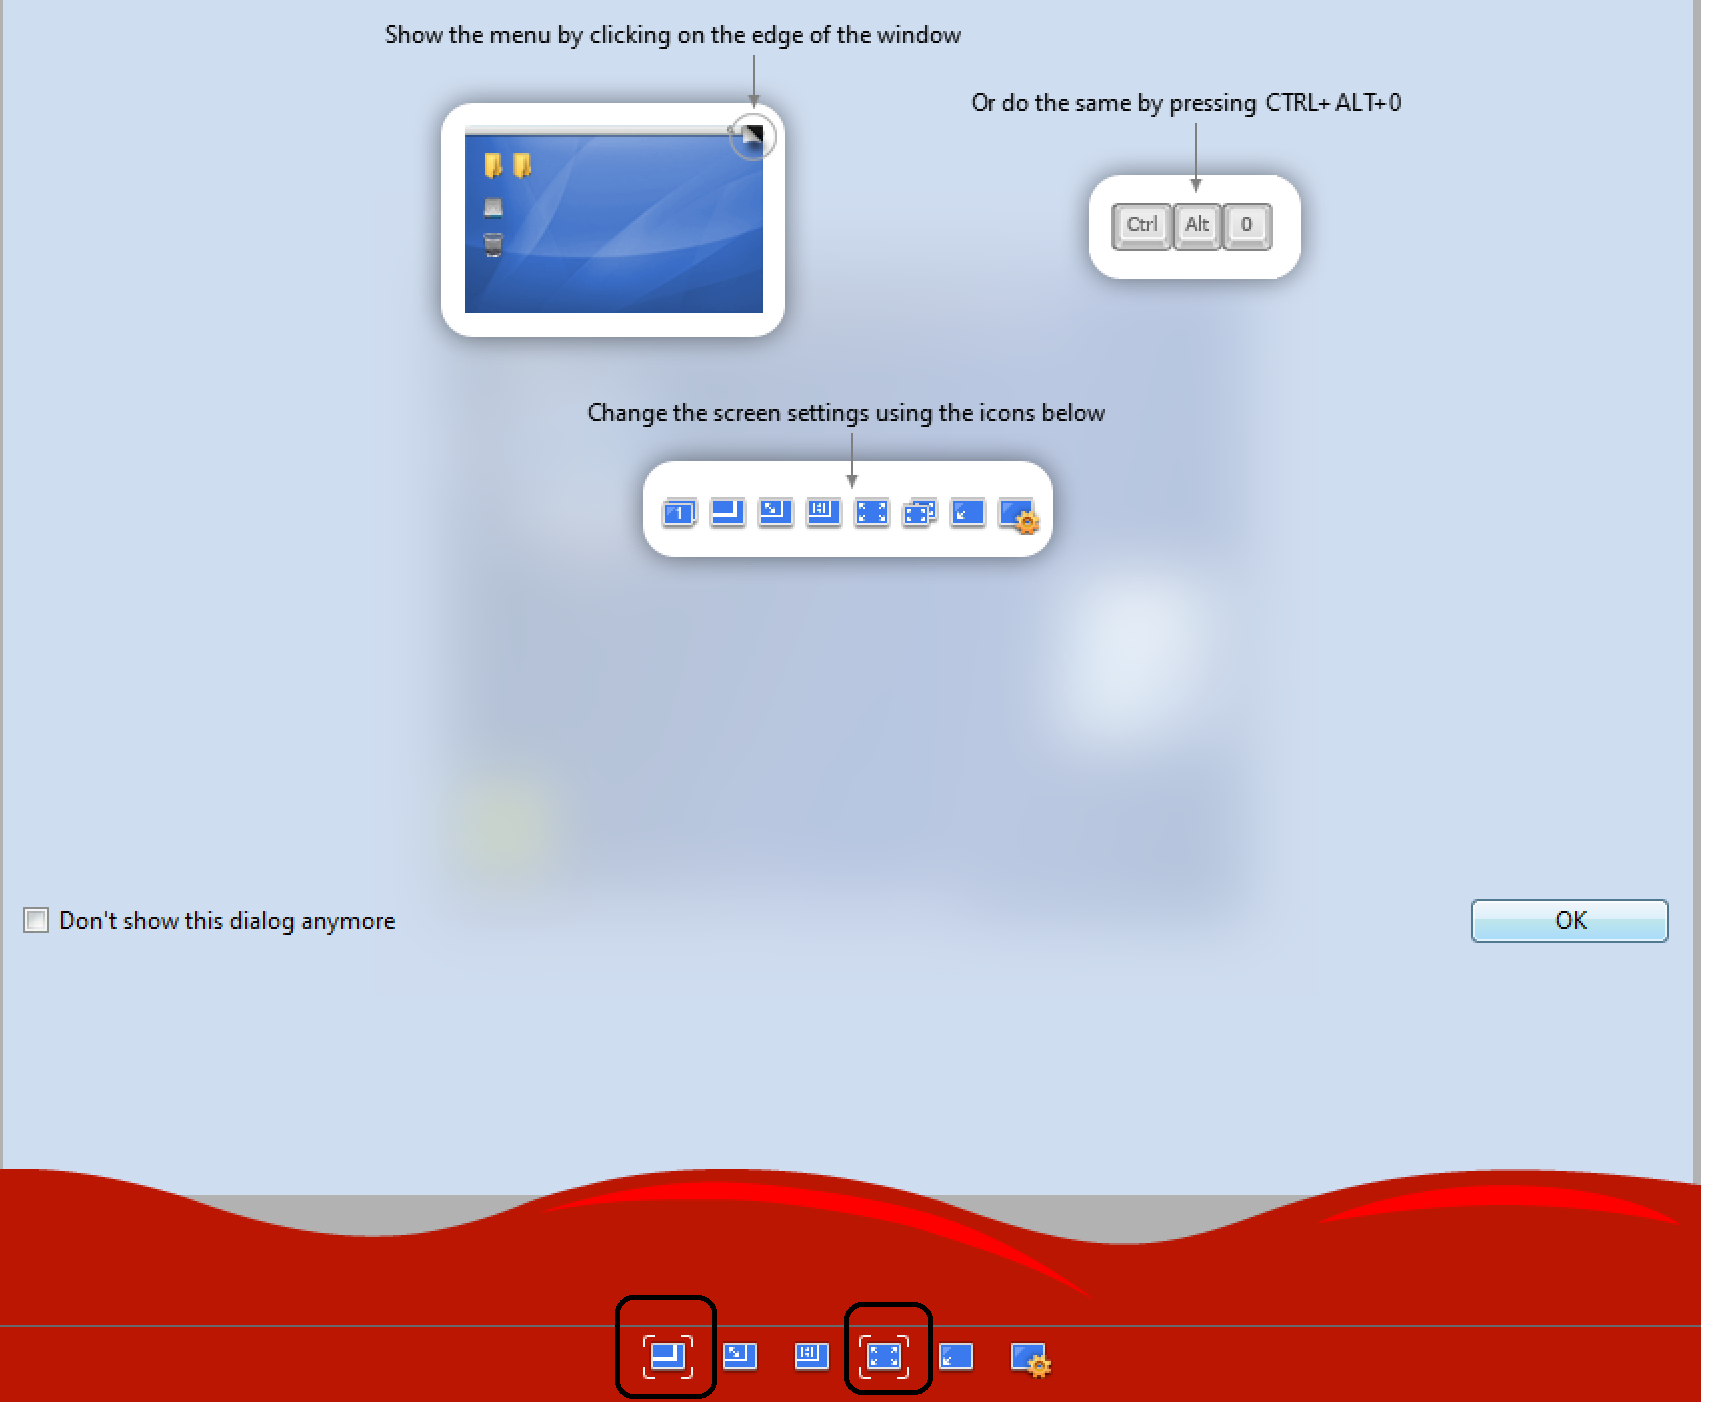
\includegraphics[width=240pt]{images/slika6} 	
	
\end{frame}	


\begin{frame}{Define remote desktop setting}
	
	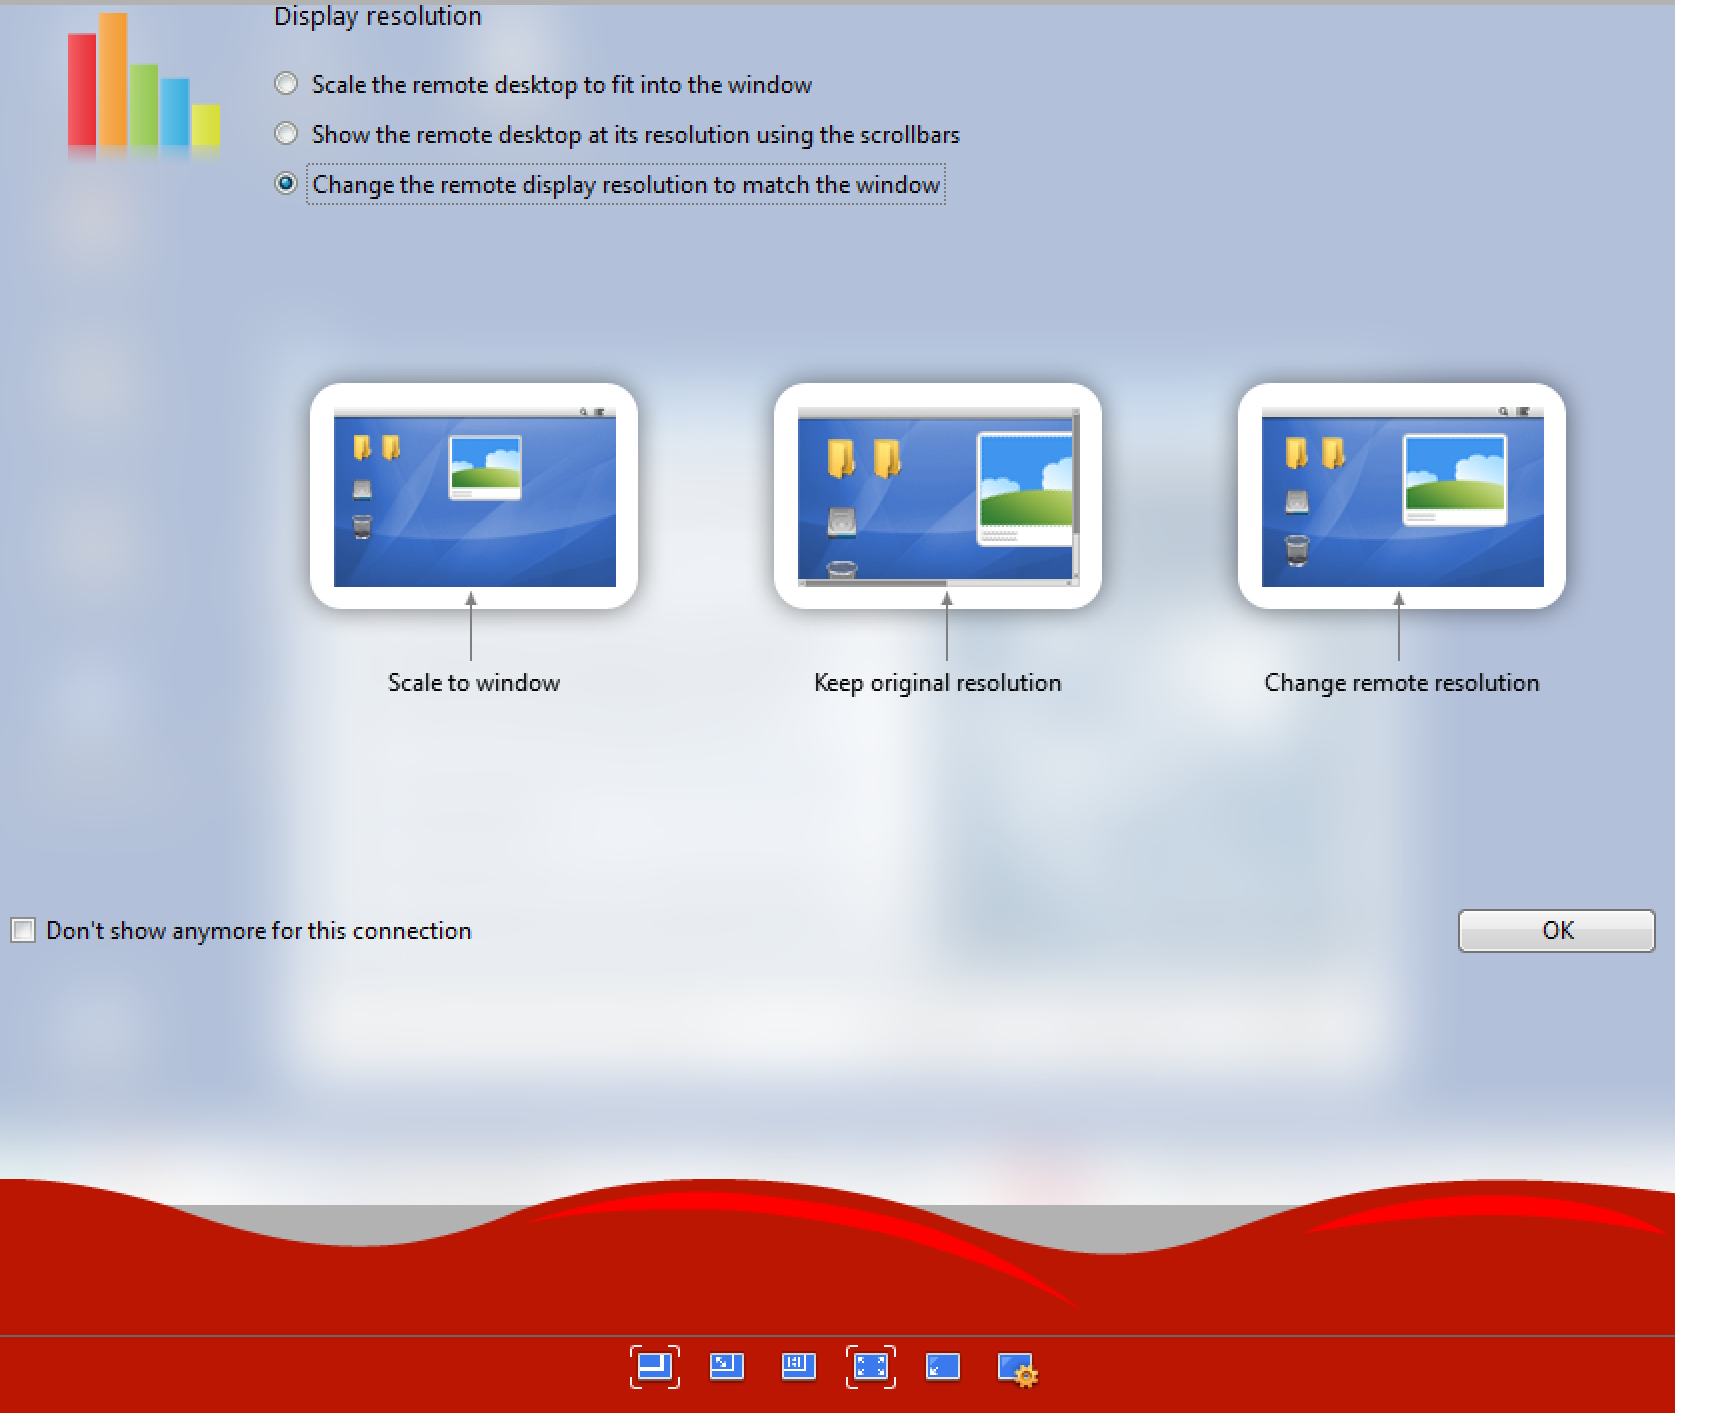
\includegraphics[width=240pt]{images/slika7} 	
	
\end{frame}	




\subsection{Run R and Rstudio on HPC}


\begin{frame}{Konzola/console/terminal window}
	Open console and type 
	\begin{itemize}
		\item {\tt module load R}
		\item {\tt R}
	\end{itemize}
	
	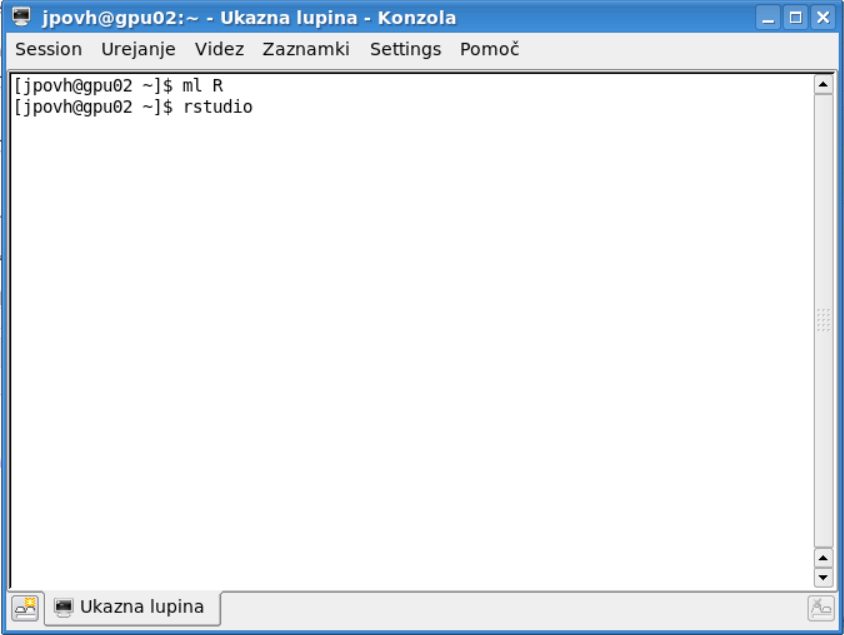
\includegraphics[width=200pt]{images/slika9} 	
\end{frame}




\begin{frame}[fragile]{Connect to compute node}
	\begin{block}{Type to console}\tiny
		\begin{lstlisting}[basicstyle=\color{blue}\tiny\ttfamily,language=R,escapeinside=`']
			LD_PRELOAD= srun -p haswell --pty --x11 bash -i 
			module load RStudio-Server/2022.07.2-576-foss-2022a-Java-11-R-4.2.1
			module help RStudio-Server/2022.07.2-576-foss-2022a-Java-11-R-4.2.1
		\end{lstlisting}
	\end{block}\pp 
	
	Copy the following text to command line\\
	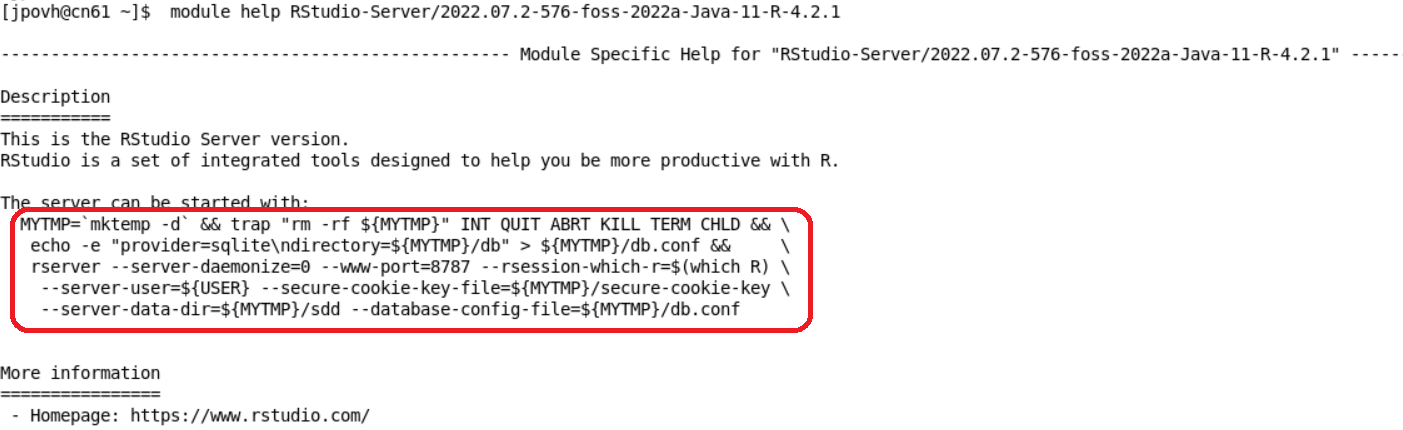
\includegraphics[width=240pt]{images/slika10} 	
\end{frame}



\begin{frame}{Run Rstudio on compute node}
	\begin{itemize}
		\item open web browser (chrome or firefow)
		\item type in {\tt http://cnXX:8787/} - XX is the name of compute node where you are.
		\item Note that both Rstudios (on login and compute node) can not run in parallel - only one.
		\\
		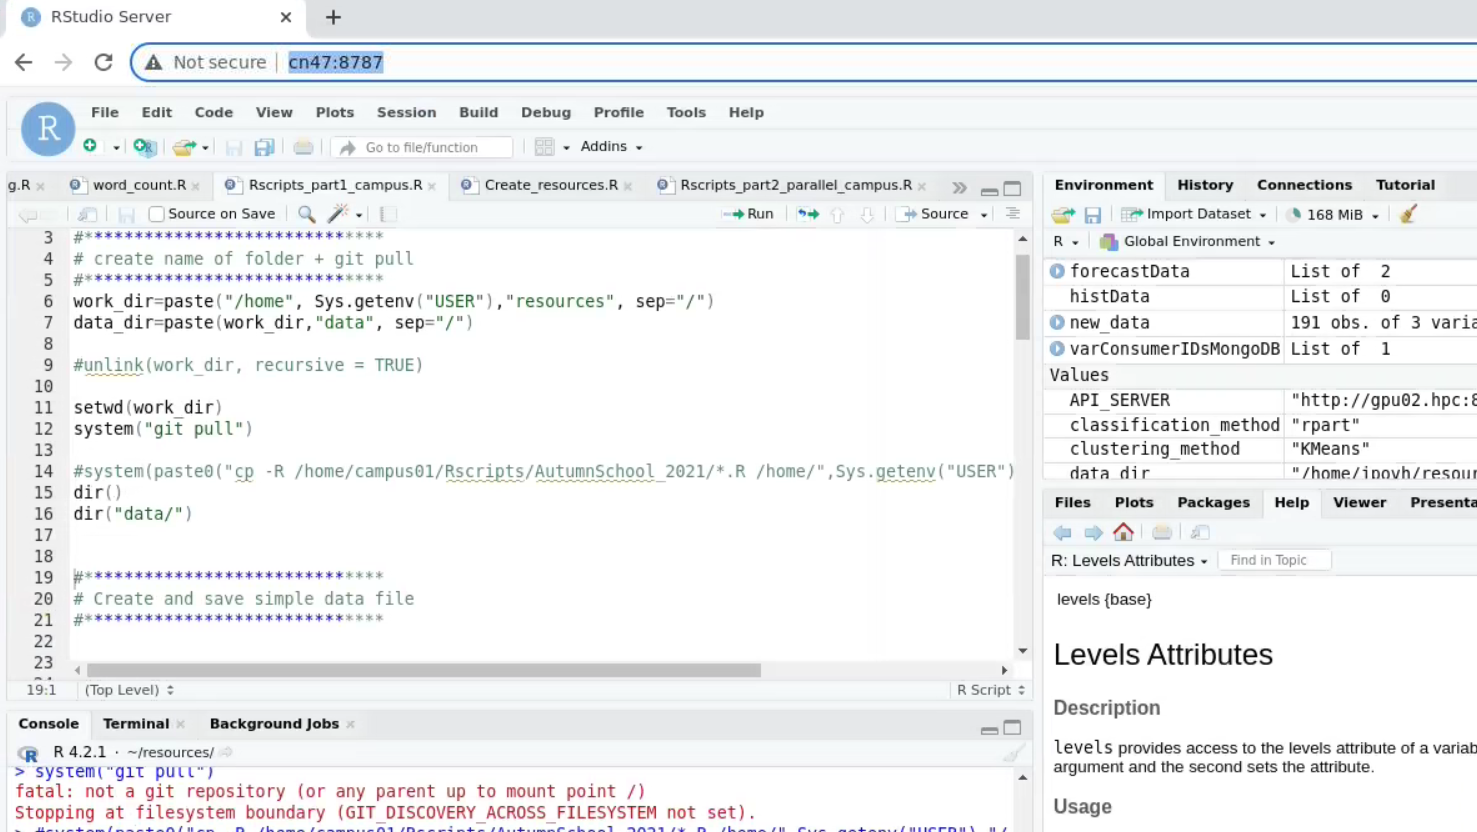
\includegraphics[width=240pt]{images/slika11} 			
		
	\end{itemize}
\end{frame}


\begin{frame}[fragile]{GITHUB}
	Clone data for today  from GITHUB
	
	\verb|https://github.com/janezpovh/Parallel_R_Jan_24.git|
	
	\end{frame}
	
\end{comment}

	
	\begin{frame}[fragile]
\frametitle{Creating the first script file}
\begin{block}{Create and save simple data file}\tiny
	\begin{lstlisting}[basicstyle=\color{blue}\tiny\ttfamily,language=R,escapeinside=`']
		N=1000;
		Data=data.frame(group=character(N),ints=numeric(N),reals=numeric(N))
		Data$group=sample(c("a","b","c"), 1000, replace=TRUE);
		Data$ints=rbinom(N,10,0.5);
		Data$reals=rnorm(N);
		
		head(Data)
		Data
		
		write.table(Data, file='data/Data_Ex_1.txt', append = FALSE, dec = ".",col.names = TRUE)
		
		ls()
		rm(list = ls())
	\end{lstlisting}	
\end{block}

\vspace{-.2cm}
\end{frame}


\begin{frame}[fragile]
\frametitle{Load and analyse the data}
\begin{block}{Load data}\scriptsize
	\begin{lstlisting}[basicstyle=\color{blue}\tiny\ttfamily,language=R,escapeinside=`']
		Data_read<-read.table(file='data/Data_Ex_1.txt',header = TRUE)
		# first few rows
		head(Data_read)
		#10 th row
		Data_read[10,]
		# column group
		Data_read$group
		Data_read[,1]		
	\end{lstlisting}
\end{block}

\end{frame}



\begin{frame}[fragile]
\frametitle{Analyse the data}
\begin{block}{Simple analysis}\scriptsize
	\begin{lstlisting}[basicstyle=\color{blue}\tiny\ttfamily,language=R,escapeinside=`']
		# compute means and counts by groups
		group count_ints mean_ints
		a | 337 | 5.014837
		b | 338 | 5.032544
		c | 325 | 4.990769
		
		# primitive solution
		Group_lev=levels(Data_read$group)
		
		Tab_summary=data.frame(group=character(3),count_ints=integer(3),mean_ints=numeric(3))
		Tab_summary$group<-Group_lev
		for (i in c(1:3)){
			sub_data = subset(Data_read,group==Group_lev[i])
			Tab_summary$count_ints[i]<-nrow(sub_data)
			Tab_summary$mean_ints[i]<-mean(sub_data$ints)
		}
	\end{lstlisting}
\end{block}

\end{frame}


\begin{comment}
	
\begin{frame}[fragile]
\frametitle{Analyse the data with {\tt dplyr, magrittr}}
\begin{itemize}\scriptsize
	\item Library {\tt dplyr}: ''select", "filter", "group\_by","arrange", "mutate" and ''summarize".
	\item Library {magrittr}: "\%>\%"
\end{itemize}
\begin{block}{{\tt dplyr}}\tiny
	\begin{lstlisting}[basicstyle=\color{blue}\tiny\ttfamily,language=R,escapeinside=`']
		llibrary(dplyr)
		library(magrittr)
		Tab_summary1<-group_by(Data_read,group) %>% dplyr::summarise(count_ints=n(),mean_ints=mean(ints))
		
		# other operations on rows and columns
		Data_read_group_ints<-Data_read %>% select(group,ints)
		# add new variable reals/ints
		Data_read<-mutate(Data_read,ratio=reals/ints)
		Data_read<-Data_read %>% mutate(ratio1=ints/reals)
		#arrange
		#sort accordind to increasing group
		Data_read<-Data_read %>% arrange(desc(group))
		Data_read<-Data_read %>% arrange(group)
	\end{lstlisting}
\end{block}

\end{frame}

\end{comment}





\begin{frame}[fragile]
\frametitle{Analyze the data by  {\tt split, aggregate}}
\begin{block}{{\tt split, aggregate}}\tiny
	\begin{lstlisting}[basicstyle=\color{blue}\tiny\ttfamily,language=R,escapeinside=`']
		s <- split(Data_read, Data_read$group)
		Tab_summary1<-cbind(aggregate(ints~group,data = Data_read,FUN=length),aggregate(ints~group,data = Data_read,FUN=mean))
		Tab_summary1<-Tab_summary1[,-3]
	\end{lstlisting}
\end{block}

\end{frame}




%\subfile{sections/01_Introduction to R}




\section{Parallel R within one node}


	
	\begin{frame}[fragile]{What system do I have}
		\begin{block}{How many cores}\tiny
			\begin{verbatim}
library(parallel)
detectCores()
> detectCores()
[1] 20
			\end{verbatim}
		\end{block}\pp
		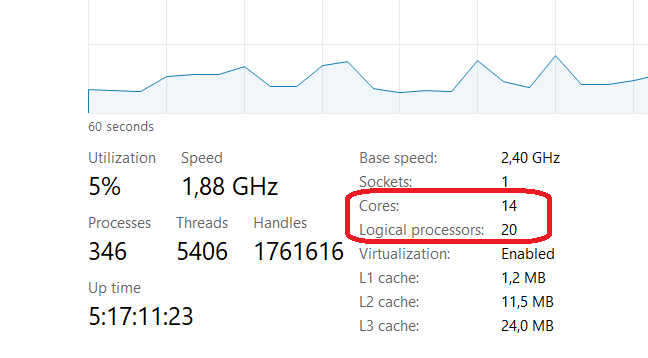
\includegraphics[width=240pt]{images/cpu_laptop} 	
	\end{frame}
	

	


\subsection{Advanced and Big data management with R}


\begin{frame}{Speed up without paralelization - vectorization}
	\CoG{Vectorization:}
	\begin{itemize}
		\item a programming technique used to avoid explicit loops in order to improve the performance and readability of code.
		\item a function can be called on a vector and operate on each element, rather than requiring a loop across elements
		\item \CoG{Example} Use {\tt sum()} or {\tt mean()} instead of loop variant.
	\end{itemize}
	
\end{frame}


\begin{frame}{Speed up without paralelization - vectorization}
	\CoG{Vectorization:}
	\begin{itemize}
		\item vectorization is faster: R is an interpreted language and not a compiled one:
		\begin{itemize}
			\item 		R needs to repeatedly interpret what your code means for each iteration of the loop;
			\item each iteration of the for loop requires indexing into the main object using the subset function.
		\end{itemize}
		\item Vectorised functions  loop over and repeatedly indexes the main object,  but this is done in the compiled language C and has been optimized to take advantage of the fact that the elements of a vector are contiguous in memory.
	\end{itemize}
	
\end{frame}



\begin{frame}[fragile]{Benchmarking}
Let us benchmark a loop and vectorised function:
	\begin{block}{{\tt Benchmarking}}\scriptsize
		\begin{lstlisting}[basicstyle=\color{blue}\tiny\ttfamily,language=R,escapeinside=`']
# Library for timing comparison
library(microbenchmark)

x <- 1:100000
microbenchmark(a = sum(x),
b = {
	s0 <- 0
	for (i in seq_along(x)) {
		s0 <- s0 + x[i]
	}
})
		\end{lstlisting}
\end{block}
\end{frame}



\begin{frame}[fragile]{{\tt apply, lapply, sapply}}
These are not typical vectorised functions - they are  “loop-hiding”, since they  contain implicit loops. {\tt apply} actually has a loop in its {\tt R} code. 
	\begin{block}{{\tt apply, lapply, sapply}}\scriptsize
		\begin{lstlisting}[basicstyle=\color{blue}\tiny\ttfamily,language=R,escapeinside=`']
apply(X, MARGIN, FUN)
Here:
-x: an array or matrix
-MARGIN=1: the manipulation is performed on rows
-MARGIN=2: the manipulation is performed on columns
-MARGIN=c(1,2): the manipulation is performed on rows and columns
-FUN: tells which function to apply. Built functions like mean, median, sum, min, max and even 
user-defined functions can be applied
		\end{lstlisting}
	\end{block}
\end{frame}


\begin{frame}[fragile]{{\tt apply}}
	For data constructed above ({\tt Data\_read}) compute row and columns means using {\tt apply} \pp 
	\begin{block}{{\tt apply}}\scriptsize
		\begin{lstlisting}[basicstyle=\color{blue}\tiny\ttfamily,language=R,escapeinside=`']
Data_read<-read.table(file='data/Data_Ex_1.txt',header = TRUE)

Data_col_means_1 <- colMeans(Data_read[,-1])
Data_col_means_2 <- apply(Data_read[,-1],2,FUN =mean)

Data_row_means_1 <- rowMeans(Data_read[,-1])
Data_row_means_2 <- apply(Data_read[,-1],1,FUN =mean)

Data_both_squares <- apply(Data_read[,-1],c(1,2),FUN = function(x) return(x^2))
		\end{lstlisting}
	\end{block}
\end{frame}



\begin{frame}[fragile]{{\tt lapply}}
	
	\begin{itemize}
		\item {\tt lapply} function takes list, vector or data frame  as input and returns only list as output
		\item {\tt sapply}  function takes list, vector or data frame  as input. It is similar to lapply function but returns only vector as output.
		
	\end{itemize}
	
	For data constructed above ({\tt Data\_read}) compute row and columns sums using {\tt lapply} \pp 
	\begin{block}{{\tt lapply}}\scriptsize
		\begin{lstlisting}[basicstyle=\color{blue}\tiny\ttfamily,language=R,escapeinside=`']
Data_col_sums_1 <- apply(Data_read[,-1],2,FUN =sum)
Data_col_sums_2 <- lapply(Data_read[,-1],FUN =sum)

typeof(Data_col_sums_1)  
typeof(Data_col_sums_2)  


Data_abs <- lapply(Data_read[,-1],FUN =abs)
Data_sq <- lapply(Data_read[,-1],FUN = function(x){x^2})

typeof(Data_abs)
length(Data_abs)
		\end{lstlisting}
	\end{block}
\end{frame}



\begin{frame}[fragile]{{\tt sapply}}
	For data constructed above ({\tt Data\_read}) compute row and columns sums using {\tt sapply} \pp 
	\begin{block}{{\tt sapply}}\scriptsize
		\begin{lstlisting}[basicstyle=\color{blue}\tiny\ttfamily,language=R,escapeinside=`']
Data_col_sums_1 <- apply(Data_read[,-1],2,FUN =sum)
Data_col_sums_2 <- lapply(Data_read[,-1],FUN =sum)
Data_col_sums_3 <- sapply(Data_read[,-1],FUN =sum)

typeof(Data_col_sums_1)  
typeof(Data_col_sums_2)  
typeof(Data_col_sums_3)  


Data_col_sums_4 <- lapply(list(Data_read$ints,Data_read$reals),FUN =sum)
Data_col_sums_5 <- sapply(list(Data_read$ints,Data_read$reals),FUN =sum)
Data_col_len_1 <- lapply(list(Data_read$ints,Data_read$reals),FUN =length)
Data_col_len_2 <- sapply(list(Data_read$ints,Data_read$reals),FUN =length)
		\end{lstlisting}
	\end{block}
\end{frame}





\begin{frame}[fragile]{{\tt for} loop}
	Let us compute sums of all elements of $K$ random matrices of order  $N\times N$
	\begin{block}{{\tt for}}\scriptsize
		\begin{lstlisting}[basicstyle=\color{blue}\tiny\ttfamily,language=R,escapeinside=`']
N=1000
K=60
set.seed(2021)
sum_rand=rep(0,K-1);
tic()
time_for_sys=system.time({
	for (i in c(1:K)){
		A=rand(N,N)
		sum_rand[i]=sum(A)
	}
})
time_for=toc()
		\end{lstlisting}
	\end{block}
\end{frame}



\begin{frame}[fragile]{ {\tt foreach do} loop}
	Let us compute sums of all elements of $K$ random matrices of order  $N\times N$
	\begin{block}{{\tt for}}\scriptsize
		\begin{lstlisting}[basicstyle=\color{blue}\tiny\ttfamily,language=R,escapeinside=`']
set.seed(2021)
sum_rand=rep(0,K-1);
tic()
time_foreach_sys=system.time({
	foreach (i = c(1:K)) %do% {
		A=rand(N,N)
		sum_rand[i]=sum(A)
	}
})
time_foreach=toc()
		\end{lstlisting}
	\end{block}
\end{frame}



\begin{frame}{Libraries {\tt parallel, doParallel}}
	\begin{itemize}
		\item {\tt parallel} package comes in the base R installation
		\item {\tt parallel} works great for any task that you pass to  the apply family (e.g., lapply becomes parLapply). 
		\item {\tt doParallel} package works great when you want to use parallel variant of for-loops (foreach--do), and might be a little easier to use.
	\end{itemize}
\end{frame}

%\end{document}






\begin{frame}[fragile]{{\tt doParallel}}
\begin{itemize}\small 
\item 	This library 
	is meant for use with {\tt foreach}, which lets you use a particular type of for-loop, that looks like:
	\begin{lstlisting}[basicstyle=\color{blue}\tiny\ttfamily,language=R,escapeinside=`']
		foreach(i=list_of_elements) %do% {thing with i}.
	\end{lstlisting}
	\pp 
	\item 
	{\tt Foreach} allows this to be parallelized, using {\tt dopar}:
	\begin{lstlisting}[basicstyle=\color{blue}\tiny\ttfamily,language=R,escapeinside=`']
		foreach(i=listOfThings) %dopar% {thing with i}.
	\end{lstlisting}
	\pp 
	\item Note that: 
	parallelization with {\tt dopar} depends on which backend you use. 
	\begin{itemize}
		\item 
		{\tt doParallel} is one such backend - it tells {\tt foreach} to use {\tt parallel}. 
		\item There are others:  {\tt doFuture, doMPI} (another parallel backend, using message passing interface), {\tt doSnow} (another backend, using the {\tt  snow} package for creating parallel processes),...
		\item By default, {\tt doParallel} uses multicore functionality on Unix-like systems and snow functionality on Windows.
		
	\end{itemize}
\end{itemize}

\end{frame}




\begin{frame}[fragile]{ Parallel {\tt foreach-dopar} loop}
Let us compute sums of all elements of $K$ random matrices of order  $N\times N$ using {\tt foreach ...dopar} from {\tt foreach} and {\tt doParallel}
\begin{block}{{\tt for}}\scriptsize
	\begin{lstlisting}[basicstyle=\color{blue}\tiny\ttfamily,language=R,escapeinside=`']
N=3000
set.seed(2021)
sum_rand=rep(0,11);
tic()
foreach (i = c(1:12)) %dopar% {
	A=randn(N,N)
	sum_rand[i]=sum(A)
}
time_foreach_dopar=toc()
	\end{lstlisting}
\end{block}
\pp
Do you observe any difference?
\end{frame}



\begin{frame}[fragile]{Creating cluster with {\tt doParallel}}
	\begin{itemize}
		\item Option 1: (use {\tt doParallel})
\begin{block}{Create cluster}\scriptsize
	\begin{lstlisting}[basicstyle=\color{blue}\tiny\ttfamily,language=R,escapeinside=`']
clust <- makeCluster(n_cores-1)  
registerDoParallel(clust)  
getDoParName()
.
.
stopCluster(clust)
#registerDoSEQ()  # alternative - register sequential mode
	\end{lstlisting}
\end{block}
\end{itemize}
\end{frame}



\begin{frame}[fragile]{Creating cluster with {\tt doParallel}}
	\begin{itemize}
		\item Option 2: use {\tt parallel}		
		\begin{block}{Create cluster}\scriptsize
			\begin{lstlisting}[basicstyle=\color{blue}\tiny\ttfamily,language=R,escapeinside=`']
registerDoParallel(cores=n_cores-1)
getDoParName()
.
.
registerDoSEQ()  # alternative - register sequential mode
			\end{lstlisting}
		\end{block}
		\item In linux: 
		\begin{itemize}
			\item the first option uses SNOW library and and utilizes {\tt parallel::parLapply()}
			\item the second creates FORK cluster and uses MULTICORE library (it effectively utilizes {\tt parallel::mclapply()}). 
		\end{itemize}
		\item In windows: both use SNOW. They create PSOCK clusters and basically utilize {\tt parallel::parLapply()}
		
	\end{itemize}
\end{frame}


\begin{frame}[fragile]{ Parallel {\tt foreach dopar} loop - option 1}
Let us compute sums of all elements of $K$ random matrices of order  $N\times N$ using {\tt foreach ...dopar} from {\tt foreach, doParallel}. Create cluster!
\begin{block}{{\tt Option 1}}\scriptsize
	\begin{lstlisting}[basicstyle=\color{blue}\tiny\ttfamily,language=R,escapeinside=`']
set.seed(2021)
clust <- makeCluster(n_cores-1)  
registerDoParallel(clust)  # use multicore, set to the number of our cores - needed for foerach dopar
getDoParName()
sum_rand=rep(0,K-1);
tic()
time_foreachdopar_1_sys=system.time({
	print("for each-dopar (cluster allocated)")
	foreach (i = c(1:K)) %dopar% {
		library(pracma)
		A=rand(N)
		sum_rand[i]=sum(A)
}}
)
time_foreach_dopar_1=toc()
stopCluster(clust)
\end{lstlisting}
\end{block}
\end{frame}


\begin{frame}[fragile]{ Parallel {\tt foreach dopar} loop - option 2}
	Let us compute sums of all elements of $K$ random matrices of order  $N\times N$ using {\tt foreach ...dopar} from {\tt foreach, doParallel}. Create cluster!
	\begin{block}{{\tt Option 2}}\scriptsize
\begin{lstlisting}[basicstyle=\color{blue}\tiny\ttfamily,language=R,escapeinside=`']
set.seed(2021)
registerDoParallel(n_cores-1)  # use multicore, set to the number of our cores - needed for foerach dopar
getDoParName()
sum_rand=rep(0,K-1);
tic()
time_foreachdopar_2_sys=system.time({
	print("for each-dopar (cluster allocated)")
	foreach (i = c(1:K)) %dopar% {
		library(pracma)
		A=rand(N)
		sum_rand[i]=sum(A)
}}
)
time_foreach_dopar_1=toc()
registerDoSEQ()   #this registers sequential mode - equivalent
\end{lstlisting}
	\end{block}
\end{frame}



\begin{frame}[fragile]{Timings}
	Timings
	\begin{verbatim}
                               user.self  sys.self  elapsed
time_for_sys                   4.16       0.50      4.93    
time_for_each_sys              4.21       0.37      4.92    
time_for_each_dopar_sys        4.11       0.55      4.98    
time_for_each_dopar_1_sys      0.13       0.01      1.90    
time_for_each_dopar_2_sys      0.11       0.00      1.80    
	\end{verbatim}
\end{frame}


\begin{frame}{Library {\tt parallel}}
\small 
\begin{itemize}
	\item encapsulates existing libraries {\tt multicore, snow}
	\item {\tt multicore}  functionality supports multiple workers only on those operating systems that support the  {\bf fork} system call - this excludes Windows. 
	
	\item two ways of parallelization:
	\begin{itemize}
		\item 
		The \CoG{socket} approach:  launches a new version of R on each core via networking (e.g. the same as if you connected to a remote server), but the connection is happening all on your own computer.
		\begin{itemize}
			\item pros: (i) Works on any system (including Windows); (ii) Each process on each node is unique so it can’t cross-contaminate.
			\item cons: (i) Each process is unique so it will be slower
			(ii) Things such as package loading need to be done in each process separately. Variables defined on your main version of R don’t exist on each core unless explicitly placed there.
			(iii) More complicated to implement.
		\end{itemize}
		\item use {\tt parLapply, parSapply}
		
		
	\end{itemize}
	
\end{itemize}

\end{frame}



\begin{frame}{Library {\tt parallel}}
\small 
\begin{itemize}
	
	\item The \CoG{forking} approach copies the entire current version of R and moves it to a new core.
	\begin{itemize}
		\item      (i) Faster than sockets.
		(ii) Because it copies the existing version of R, your entire workspace exists in each process.
		(iii) Easy to implement.
		\item 
		Cons (i) Only works on POSIX systems (Mac, Linux, Unix, BSD) and not Windows.
		(ii) it can cause issues specifically with random number generation 
		or when running in a GUI (such as RStudio). This doesn’t come up often.
	\end{itemize}
	\item use {\tt mclapply}
\end{itemize}

\end{frame}

\begin{frame}[fragile]{ Parallel versions of {\tt lapply}}
By using library {\tt parallel } and {\tt parSapply, mclapply}	compute sums of all elements of $K$ random matrices of order  $N\times N$. Create cluster!
\begin{block}{ parallel versions of {\tt apply}}\tiny
	\begin{lstlisting}[basicstyle=\color{blue}\tiny\ttfamily,language=R,escapeinside=`']
mat_sum<-function(x){
	library(pracma)
	A=rand(x)
	return(sum(A))
}

time_lapply<-system.time({
	set.seed(2021)
	sum_rand_lapply=lapply(rep(N,K),FUN=mat_sum)
})

time_sapply<-system.time({
	set.seed(2021)
	sum_rand_sapply=sapply(rep(N,K),FUN=mat_sum)
})
		
	\end{lstlisting}
\end{block}
\end{frame}

\begin{frame}[fragile]{ Parallel versions of {\tt lapply}}
\begin{block}{ parallel versions of {\tt apply}}\tiny
	\begin{lstlisting}[basicstyle=\color{blue}\tiny\ttfamily,language=R,escapeinside=`']
#forking
time_mcLapply<-system.time({
	set.seed(2021)
	sum_rand_mcLapply=mclapply(X=rep(N,K),FUN=mat_sum,mc.cores = n_cores)
})

# socketing
clust <- makeCluster(n_cores, type="PSOCK")  
time_parLapply<-system.time({
	set.seed(2021)
	sum_rand_parLapply=parLapply(clust,rep(N,K),fun=mat_sum)
})
stopCluster(clust)

clust <- makeCluster(n_cores, type="PSOCK")  
time_parSapply<-system.time({
	set.seed(2021)
	sum_rand_parSapply=parSapply(clust,rep(N,K),FUN=mat_sum)
})
stopCluster(clust) 	
	\end{lstlisting}
\end{block}
\end{frame}

\begin{frame}[fragile]{ Parallel versions of {\tt lapply}}
\begin{block}{ parallel versions of {\tt apply} - 2 cores}\tiny
	\begin{lstlisting}[basicstyle=\color{blue}\tiny\ttfamily,language=R,escapeinside=`']
		times_apply<-rbind(time_lapply,time_sapply,time_parLapply,time_parSapply,time_mcLapply) 
		
		> times_apply[,1:3]
                   user.self  sys.self elapsed
time_lapply        1.725    0.062   1.787
time_sapply        1.782    0.052   1.832
time_parLapply     0.006    0.001   0.977
time_parSapply     0.005    0.000   0.961
time_mcLapply      0.004    0.007   0.937	
\end{lstlisting}
\end{block}
\end{frame}

\begin{frame}{Summary: libraries for shared memory parallelization in {\tt R}}
\begin{itemize}
	\item Parallel for-loop ({\tt foreach...dopar}). Cluster created by {\tt registerDoParallel(N)} and {\tt registerDoSEQ()}. Library {\tt foreach, doParalel} needed.
	\item Parallel {\tt apply}: {\tt parLapply, parSapply, mcLapply} need library {parallel}. 
\end{itemize}
\end{frame}




\begin{frame}[fragile]{Very parallelizable task}
\begin{block}{Perfectly parallelizable computing task}\tiny
	\begin{lstlisting}[basicstyle=\color{blue}\tiny\ttfamily,language=R,escapeinside=`']
# simple very parallel
library(parallel)
library(tictoc)

f <- function(...) {
	Sys.sleep(1) 
	"DONE"
}


for (p in 1:8) {
	t <- system.time(
	mclapply(1:25, f, mc.cores = p)
	)	
	cat("workers =", p,
	" elapsed =", t["elapsed"], "\n")
}

workers = 1  elapsed = 25.005 
workers = 2  elapsed = 13.008 
workers = 3  elapsed = 9.005 
workers = 4  elapsed = 7.006 
workers = 5  elapsed = 5.013 
workers = 6  elapsed = 5.006 
workers = 7  elapsed = 4.01 
workers = 8  elapsed = 4.005 

	\end{lstlisting}
\end{block}
\end{frame}


\begin{frame}[fragile]{Not so parallelizable task}
	\begin{block}{Weakly parallelizable computing task}\tiny
		\begin{lstlisting}[basicstyle=\color{blue}\tiny\ttfamily,language=R,escapeinside=`']
# simple very parallel
library(parallel)
library(tictoc)

g <- function(...) {
	sum(rnorm(1e7))
}

for (p in 1:8) {
	t <- system.time(
	mclapply(1:25, g, mc.cores = p)
	)	
	cat("workers =", p,
	" elapsed =", t["elapsed"], "\n")
}


workers = 1  elapsed = 10.431 
workers = 2  elapsed = 5.524 
workers = 3  elapsed = 5.634 
workers = 4  elapsed = 5.667 
workers = 5  elapsed = 5.624 
workers = 6  elapsed = 5.886 
workers = 7  elapsed = 5.594 
workers = 8  elapsed = 5.575 
			
		\end{lstlisting}
	\end{block}
\end{frame}


\begin{frame}[fragile]{Cross-validation of models}
\begin{itemize}
	\item 	Suppose we want to cretae $N$ GLM models, where training data sets is random sample of size 70\%, and test data sets is the remaing set. 
	\item If $N=10$ and we use 10\% training set, we have the usual 10-fold cross-validation.
	\item We do it on dataset {\tt K\_data\_clean.txt}.
	\item Use {\tt R} script {\tt parallel\_cross-validation.R}
	\item Timings with 10 cores
		\begin{verbatim}
		            user.self  sys.self   elapsed
        time_ser    139.71     0.11       141.89    
        time_par      0.76     0.13        30.82    
 \end{verbatim}
\end{itemize}
\end{frame}

%\section{Advanced and Big data management with R}
%\subfile{sections/02_advanced data analysis with R}

\begin{comment}
	
	
\section{Parallelization with Rmpi}
%\subfile{sections/04_Rmpi}




	
	\begin{frame}[fragile]{What  is Rmpi}
		\begin{itemize}
			\item Rmpi library: Interface for MPI (Message Passing Interface) in R.
			\item Enables parallel and distributed computing in the R programming language.
			\item Facilitates communication and coordination between R processes across multiple nodes.
			\item Particularly useful for parallelizing computationally intensive tasks like simulations or data processing.
			\item Users can harness the power of parallel computing for improved performance in certain applications.
			\item Latest version from Dec 2023, see \url{https://cran.r-project.org/web/packages/Rmpi/Rmpi.pdf}
		\end{itemize}
	\end{frame}
	
	
	\begin{frame}{Few basic command}
		\begin{itemize}
			\item {\tt Rmpi::mpi.comm.size(0)}: returns the number of active processes in current computing task/job
			\item {\tt Rmpi::mpi.comm.rank(0)}: returns the ID of current process (number from $\{0,1,2,\ldots,\mbox{size}-1\}$ 
			\item {\tt Rmpi::mpi.get.processor.name()} - returns the name of compute node where the process runs.
		\end{itemize}
	\end{frame}
	
	
		
	
	\begin{frame}[fragile]{Hello word example}
		\begin{block}{Compute smallest eigenvalue of $n\times n$ random symmetric matrices}\tiny
			\begin{lstlisting}[basicstyle=\color{blue}\tiny\ttfamily,language=R,escapeinside=`']
				library(Rmpi)
				n=30
				size <- Rmpi::mpi.comm.size(0)
				rank <- Rmpi::mpi.comm.rank(0)
				host <- Rmpi::mpi.get.processor.name()
				if (rank == 0){
					cat("size ","rank ","host ","max_eigen_value\n")
					cat(size,rank,host,"NaN\n")
				} else {
					where=getwd()
					A=matrix(rnorm(n^2),nrow=n)
					A=A+t(A)
					a = max(eigen(A)$values)
					cat(size,rank,host,a,"\n")    
				}
			\end{lstlisting}
		\end{block}
	\end{frame}
	
	
	\begin{frame}[fragile]{How to distribute this task across cluster}
		\begin{itemize}
			\item Save the scripts from previous slide into separate file, called e.g. \verb|Rmpi_master_slave.R|
			\item  Create separate \verb|.batch| file, where the parallelization is defined, e.g., 
			\verb|Job_Rmpi_master_slave.sbatch|
		\end{itemize}
	\end{frame}
	
	
	\begin{frame}[fragile]{How to distribute this task across cluster}
		\begin{block}{Compute smallest eigenvalue of $n$ symmetric matrices of size $N\times N$}\tiny
			\begin{lstlisting}[basicstyle=\color{blue}\tiny\ttfamily,language=R,escapeinside=`']
				#!/bin/bash
				#SBATCH --export=ALL,LD_PRELOAD=
				#SBATCH --job-name Rmpi
				#SBATCH --partition=qcpu --time=02:00
				#SBATCH --nodes=2
				#SBATCH --ntasks-per-node 36 ## maximum is 36
				#SBATCH --output=logs/%x_%j.out
				#SBATCH --account dd-24-88-015
				
				## not needed module load OpenMPI/4.1.4-GCC-11.3.0
				module load R/4.1.0-foss-2021a
				srun  Rscript Rmpi_master_slave.R			
\end{lstlisting}
		\end{block}
	\end{frame}

	\begin{frame}[fragile]{Go to Barbora}
	\begin{itemize}\small
		\item Create directory\\ \verb|mkdir /home/rstudio/mnt/|
		\item copy to it files\\\tiny  \verb|Job_Rmpi_master_slave.sbatch, Rmpi_master_slave.R|
		\item \small mount this directory \\\tiny  
		\verb|sshfs -o IdentityFile=/home/rstudio/.ssh/id_ed25519 it4i-jpovh@barbora.it4i.cz:. /home/rstudio/mnt/|  OR \\
		\verb|bash barbora_mount|
		\item \small connect to barbora with ssh \\\tiny 
		\verb|ssh -i /home/rstudio/.ssh/id_ed25519 it4i-jpovh@barbora.it4i.cz|  OR \\
		\verb|bash barbora_login|
		\item \normalsize If troubles with data format\\
		\verb|sed -i 's/\r$//' <your_script.sh>|
	\end{itemize}
\end{frame}

\begin{frame}[fragile]{Connect to Barbora}
	
\includegraphics[width=200pt]{images/barbora}

\begin{itemize}
	\item 	Run \\ \small\verb|sbatch Job_Rmpi_master_slave.sbatch|
\end{itemize}


\end{frame}

	
	
	\begin{frame}[fragile]{Results in log file}
			Results in folder {\tt ~mnt/logs}.
		
		\begin{verbatim}
			[1] "size rank host max_eigen_value"
			[1] "384 0 cn48 NaN"
			[1] "384 110 cn50 8.25199803297607"
			[1] "384 173 cn52 8.01187455128492"
			[1] "384 68 cn49 8.05800653948316"
			[1] "384 200 cn53 8.81600769867893"
			[1] "384 258 cn54 8.12244071842822"
			[1] "384 332 cn55 7.61927646789373"
			[1] "384 338 cn56 4.9472190383247"
		\end{verbatim}
		
	\end{frame}
	
	
	\begin{frame}[fragile]{Connect to Barbora}
		\begin{itemize}
			\item Time needed for the job\scriptsize
			\begin{verbatim}
				[it4i-jpovh@login2.barbora ~]$ sacct --format=JobID,JobName,State,Elapsed
				JobID           JobName      State    Elapsed 
				------------ ---------- ---------- ---------- 
				717928             Rmpi  COMPLETED   00:00:08 
				717928.batch      batch  COMPLETED   00:00:08 
				717928.exte+     extern  COMPLETED   00:00:08 
				717928.0        Rscript  COMPLETED   00:00:05 				
			\end{verbatim}
			
		\end{itemize}
		
		
	\end{frame}
	
	\begin{frame}[fragile]{How parallelise without slurm?}
		\begin{block}{Compute smallest eigenvalue of $n$ symmetric matrices of size $N\times N$}\tiny
			\begin{lstlisting}[basicstyle=\color{blue}\tiny\ttfamily,language=R,escapeinside=`']
				rm(list=ls())  # R code: parallel version 
				library(snow) 
				library(Rmpi)  
				nclus=6  
				cl <-snow::makeMPIcluster(nclus)  #alter either n or mc to affect run time 
				n=30 
				N_per_proc=100  
				#x=matrix(runif(n),n,1) 
				#x=cbind(1,x)  
				min_eig_values=function(n,N){
					a=c()
					for (ind in 1:N){
						A=matrix(rnorm(n^2),nrow=n)
						A=A+t(A)
						a[ind] = max(eigen(A)$values)
					}
					return(a)
				}  
				ptim=proc.time()[3]  
				b=clusterCall(cl,min_eig_values,n=n,N=N_per_proc)  
				b=unlist(b)
				hist(b)
				tim=proc.time()[3]-ptim  
				#Rmpi::mpi.quit()
				snow::stopCluster(cl) 
			\end{lstlisting}
		\end{block}
	\end{frame}
	

\end{comment}

% Parallel R course: 2026 update module
% Insert this file after the existing single-node parallel section and before Rcpp.
% Requires: listings, xcolor, hyperref. Optional: booktabs.

\section{Modern parallel R workflows}

\begin{frame}{Learning objectives for the updated module}
\begin{itemize}
  \item Choose an appropriate execution model: sequential, vectorised, process-based, scheduler-based, or GPU.
  \item Use the \texttt{future} ecosystem for portable parallel code.
  \item Run reproducible parallel simulations.
  \item Scale the same computation from a workstation to a Slurm cluster.
  \item Recognise when faster I/O or an analytical database is better than adding workers.
\end{itemize}
\end{frame}

\begin{frame}{A modern performance workflow}
\begin{enumerate}
  \item Measure the real bottleneck: CPU, memory, I/O, or communication.
  \item Improve the algorithm and data representation.
  \item Use vectorised or compiled routines.
  \item Parallelise only sufficiently large, independent tasks.
  \item Scale across nodes only when one node is insufficient.
  \item Verify correctness, reproducibility, memory use, and speedup.
\end{enumerate}
\vspace{0.2cm}
\alert{Parallel execution is not automatically faster.} Startup, data transfer, serialisation, and load imbalance can dominate short tasks.
\end{frame}

\begin{frame}[fragile]{How many workers should I use?}
\begin{block}{Use the resources available to the current process}
\begin{lstlisting}[language=R]
library(parallelly)

availableCores()       # respects many scheduler/container limits
availableWorkers()     # workers visible to the current R session

detectCores()          # hardware/logical CPUs, not always usable CPUs
\end{lstlisting}
\end{block}
\begin{itemize}
  \item Logical processors are not necessarily equally fast on hybrid CPUs.
  \item On an HPC system, use the CPUs granted by the scheduler, not the whole node.
  \item Leave capacity for the operating system on an interactive workstation.
\end{itemize}
\end{frame}

\begin{frame}{Processes, threads, and oversubscription}
\begin{itemize}
  \item \textbf{R workers} are usually separate processes with separate memory.
  \item BLAS, OpenMP, \texttt{data.table}, and compiled libraries may create additional threads.
  \item Eight R workers with eight BLAS threads each can create up to 64 runnable threads.
  \item Oversubscription often reduces performance and makes timings unstable.
\end{itemize}
\vspace{0.2cm}
Practical rule: when using many R workers, initially set threaded numerical libraries to one thread per worker, benchmark, and then tune.
\end{frame}

\begin{frame}[fragile]{Benchmark elapsed time and memory}
\begin{block}{Prefer representative workloads}
\begin{lstlisting}[language=R]
library(bench)

x <- runif(1e6)
bench::mark(
  loop = {
    ans <- 0
    for (i in seq_along(x)) ans <- ans + x[[i]]
    ans
  },
  vectorised = sum(x),
  check = TRUE
)
\end{lstlisting}
\end{block}
\begin{itemize}
  \item Compare results, not just timings.
  \item Report elapsed time, memory allocation, workload size, worker count, and hardware.
\end{itemize}
\end{frame}

\subsection{The future ecosystem}

\begin{frame}{Why teach the \texttt{future} ecosystem?}
\begin{itemize}
  \item It separates \textbf{what} should be evaluated from \textbf{where and how} it runs.
  \item The computational code can remain stable while the execution plan changes.
  \item Common front ends include \texttt{future.apply}, \texttt{furrr}, and \texttt{doFuture}.
  \item Backends cover local processes, remote workers, and scheduler-managed HPC jobs.
\end{itemize}
\vspace{0.2cm}
Keep \texttt{parallel} and \texttt{foreach} in the course as foundations and legacy interfaces, but use \texttt{future} as the main portable workflow.
\end{frame}

\begin{frame}[fragile]{From sequential to parallel with one change}
\begin{block}{Portable parallel map}
\begin{lstlisting}[language=R]
library(future)
library(future.apply)

f <- function(i) {
  x <- rnorm(2e6)
  c(task = i, statistic = mean(exp(x)))
}

plan(sequential)
a <- future_lapply(1:8, f, future.seed = TRUE)

plan(multisession, workers = 4)
b <- future_lapply(1:8, f, future.seed = TRUE)

identical(a, b)
plan(sequential)
\end{lstlisting}
\end{block}
\end{frame}

\begin{frame}[fragile]{Parallel tidy workflows with \texttt{furrr}}
\begin{block}{The \texttt{purrr} interface with futures}
\begin{lstlisting}[language=R]
library(future)
library(furrr)

plan(multisession, workers = 4)

results <- future_map(
  1:20,
  ~ mean(rnorm(1e6, mean = .x)),
  .options = furrr_options(seed = 2026)
)

plan(sequential)
\end{lstlisting}
\end{block}
Use this interface when students already know \texttt{purrr::map()}.
\end{frame}

\begin{frame}[fragile]{Keep existing \texttt{foreach} code with \texttt{doFuture}}
\begin{block}{Modern backend for a familiar interface}
\begin{lstlisting}[language=R]
library(future)
library(doFuture)
library(foreach)

registerDoFuture()
plan(multisession, workers = 4)

ans <- foreach(i = 1:20,
               .combine = c,
               .options.future = list(seed = TRUE)) %dopar% {
  mean(rnorm(1e6, mean = i))
}

plan(sequential)
\end{lstlisting}
\end{block}
This provides a migration path rather than requiring an immediate rewrite of all \texttt{foreach} material.
\end{frame}

\begin{frame}{Choosing a local future plan}
\begin{itemize}
  \item \texttt{sequential}: debugging, teaching, and a reproducible baseline.
  \item \texttt{multisession}: separate R processes; portable across Windows, macOS, and Linux.
  \item \texttt{multicore}: forked processes; available on supported POSIX systems, not Windows.
  \item Explicit cluster backends: use when workers are remote or require custom startup.
\end{itemize}
\vspace{0.2cm}
For a mixed classroom, \texttt{multisession} is the safest default. Always return to \texttt{plan(sequential)} after an exercise.
\end{frame}

\subsection{Reproducibility and diagnostics}

\begin{frame}[fragile]{Reproducible parallel random numbers}
\begin{block}{Do not rely only on \texttt{set.seed()} before parallel mapping}
\begin{lstlisting}[language=R]
library(future.apply)

plan(multisession, workers = 4)
set.seed(2026)

z1 <- future_lapply(1:10, function(i) rnorm(3),
                    future.seed = TRUE)

set.seed(2026)
z2 <- future_lapply(1:10, function(i) rnorm(3),
                    future.seed = TRUE)

identical(z1, z2)
plan(sequential)
\end{lstlisting}
\end{block}
Reproducibility must hold when the worker count or backend changes.
\end{frame}

\begin{frame}{Common reasons for disappointing speedup}
\begin{itemize}
  \item Tasks are too short compared with worker startup and communication.
  \item Large global objects are copied or serialised for every task.
  \item Workers compete for memory bandwidth or disk I/O.
  \item Work is unevenly distributed among workers.
  \item Nested parallelism oversubscribes CPUs.
  \item A sequential fraction limits total speedup (Amdahl's law).
\end{itemize}
\vspace{0.2cm}
Measure serial and parallel versions using the same inputs and verify that they return equivalent results.
\end{frame}

\begin{frame}[fragile]{Chunking: amortise scheduling overhead}
\begin{block}{Prefer fewer substantial tasks to millions of tiny tasks}
\begin{lstlisting}[language=R]
library(future.apply)

plan(multisession, workers = 4)

ids <- split(1:10000, cut(1:10000, 40, labels = FALSE))
ans <- future_lapply(ids, function(block) {
  vapply(block, expensive_function, numeric(1))
})
ans <- unlist(ans, use.names = FALSE)
\end{lstlisting}
\end{block}
The best chunk size depends on task duration, variability, memory use, and backend latency.
\end{frame}

\subsection{From one node to Slurm}

\begin{frame}{A scheduler changes resource ownership}
\begin{itemize}
  \item The login node is for editing, compiling, and submitting jobs, not heavy computation.
  \item Slurm grants CPUs, memory, accelerators, nodes, and wall time to a job.
  \item R should discover and use only the resources allocated to that job.
  \item Multi-node execution adds network communication and distributed failure modes.
\end{itemize}
\end{frame}

\begin{frame}[fragile]{A minimal Slurm batch job}
\begin{block}{\texttt{run\_analysis.sbatch}}
\begin{lstlisting}[language=bash]
#!/bin/bash
#SBATCH --job-name=parallel-r
#SBATCH --nodes=1
#SBATCH --cpus-per-task=8
#SBATCH --mem=32G
#SBATCH --time=00:30:00
#SBATCH --output=logs/%x_%j.out

module load R
Rscript analysis.R
\end{lstlisting}
\end{block}
Submit with \texttt{sbatch run\_analysis.sbatch}; inspect the queue with \texttt{squeue -u \$USER}.
Adapt partition, account, module name, memory, and time to the target system.
\end{frame}

\begin{frame}[fragile]{Use Slurm through \texttt{future.batchtools}}
\begin{block}{Change the plan, not the analytical function}
\begin{lstlisting}[language=R]
library(future)
library(future.apply)
library(future.batchtools)

plan(
  future.batchtools::batchtools_slurm,
  resources = list(
    time = "00:20:00",
    mem = "4G",
    ncpus = 1
  )
)

ans <- future_lapply(files, analyse_file,
                     future.seed = TRUE)
\end{lstlisting}
\end{block}
Resource field names depend on the cluster template. Test with a small job before scaling up.
\end{frame}

\begin{frame}{Single node or multiple nodes?}
\begin{itemize}
  \item Start with one node: lower latency, simpler debugging, and usually faster data access.
  \item Use multiple nodes when memory, throughput, or turnaround requirements exceed one node.
  \item Independent simulations and file-level processing scale more easily than tightly coupled algorithms.
  \item For communication-heavy numerical algorithms, specialised MPI or distributed libraries may be more appropriate.
\end{itemize}
\end{frame}

\subsection{Data movement before parallelism}

\begin{frame}{Sometimes the bottleneck is data, not R code}
\begin{itemize}
  \item CSV parsing, repeated scans, and object copying can dominate the computation.
  \item Columnar formats such as Parquet reduce unnecessary I/O for analytical workloads.
  \item Apache Arrow supports columnar and dataset-oriented workflows.
  \item DuckDB can execute analytical SQL directly over local files and tabular data.
\end{itemize}
\vspace{0.2cm}
Before adding workers, reduce the amount of data read, copied, and returned.
\end{frame}

\begin{frame}[fragile]{Query Parquet data without loading everything}
\begin{block}{Arrow dataset with lazy filtering and aggregation}
\begin{lstlisting}[language=R]
library(arrow)
library(dplyr)

sales <- open_dataset("data/sales", format = "parquet")

summary <- sales |>
  filter(year == 2026) |>
  group_by(region) |>
  summarise(revenue = sum(amount, na.rm = TRUE)) |>
  collect()
\end{lstlisting}
\end{block}
Only call \texttt{collect()} when the reduced result is needed as an in-memory R object.
\end{frame}

\begin{frame}[fragile]{Use DuckDB for analytical queries}
\begin{block}{Push computation into an analytical database}
\begin{lstlisting}[language=R]
library(DBI)
library(duckdb)

con <- dbConnect(duckdb())
result <- dbGetQuery(con, "
  SELECT region, AVG(value) AS mean_value
  FROM read_parquet('data/*.parquet')
  GROUP BY region
")
dbDisconnect(con, shutdown = TRUE)
\end{lstlisting}
\end{block}
Compare this approach with manually splitting files among R workers.
\end{frame}

\subsection{Compiled and accelerator execution}

\begin{frame}{Four distinct acceleration strategies}
\begin{itemize}
  \item \textbf{Vectorisation}: use optimised compiled routines already available to R.
  \item \textbf{Process parallelism}: distribute independent R tasks among workers.
  \item \textbf{Compiled extensions}: move a hot loop to C++ with \texttt{Rcpp}.
  \item \textbf{Accelerators}: use GPU-aware libraries for suitable dense, batched, or model-training workloads.
\end{itemize}
These strategies can be combined, but nested parallelism and data transfers must be controlled.
\end{frame}

\begin{frame}{Extend the Mandelbrot example with \texttt{RcppParallel}}
\begin{itemize}
  \item Keep the existing three implementations: R, R with a C++ kernel, and complete C++.
  \item Add a fourth implementation using \texttt{RcppParallel::parallelFor}.
  \item Partition grid indices among threads and write each output element once.
  \item Compare elapsed time and scaling for 1, 2, 4, and 8 threads.
  \item Discuss grain size, memory bandwidth, thread safety, and reproducibility.
\end{itemize}
\end{frame}

\begin{frame}[fragile]{GPU tensors from R with \texttt{torch}}
\begin{block}{Use an accelerator-aware library rather than explicit GPU loops}
\begin{lstlisting}[language=R]
library(torch)

device <- if (cuda_is_available()) torch_device("cuda") else torch_device("cpu")

x <- torch_randn(c(4000, 4000), device = device)
y <- torch_randn(c(4000, 4000), device = device)
z <- torch_matmul(x, y)

z_cpu <- z$to(device = "cpu")
\end{lstlisting}
\end{block}
GPU speedup depends on operation size, supported kernels, device memory, and host--device transfer costs.
\end{frame}

\subsection{Updated practical exercise}

\begin{frame}{Capstone: parallel model evaluation}
\begin{enumerate}
  \item Create a fixed resampling or hyperparameter grid.
  \item Implement one deterministic function that evaluates a single grid row.
  \item Run it sequentially and verify results.
  \item Run locally with \texttt{future\_map()} or \texttt{future\_lapply()}.
  \item Run the same function through a Slurm backend.
  \item Report elapsed time, speedup, efficiency, memory, and failed tasks.
\end{enumerate}
\end{frame}

\begin{frame}[fragile]{Capstone skeleton}
\begin{block}{Backend-independent worker function}
\begin{lstlisting}[language=R]
library(future)
library(furrr)

grid <- expand.grid(
  penalty = 10^seq(-4, 1, length.out = 20),
  split = 1:10
)

evaluate_one <- function(i) {
  row <- grid[i, ]
  # fit on the training split; score on the test split
  data.frame(i = i, penalty = row$penalty,
             split = row$split, score = NA_real_)
}

plan(multisession, workers = 4)
scores <- future_map_dfr(
  seq_len(nrow(grid)), evaluate_one,
  .options = furrr_options(seed = 2026)
)
plan(sequential)
\end{lstlisting}
\end{block}
Replace the placeholder score with the course model and dataset.
\end{frame}

\begin{frame}{Updated summary}
\begin{itemize}
  \item Optimise the algorithm and data movement before parallelising.
  \item Use \texttt{parallel} to explain processes, PSOCK, and forked execution.
  \item Use \texttt{future} as the primary portable parallel interface.
  \item Treat reproducible random numbers and worker cleanup as core correctness topics.
  \item Use Slurm-aware backends for HPC scaling.
  \item Consider Arrow, DuckDB, compiled code, or GPUs when they match the bottleneck.
\end{itemize}
\end{frame}

\begin{frame}{References and documentation}
\scriptsize
\begin{itemize}
  \item Futureverse: \url{https://www.futureverse.org/}
  \item \texttt{future.batchtools}: \url{https://future.batchtools.futureverse.org/}
  \item \texttt{parallelly}: \url{https://parallelly.futureverse.org/}
  \item Arrow R documentation: \url{https://arrow.apache.org/docs/r/}
  \item DuckDB R client: \url{https://duckdb.org/docs/stable/clients/r}
  \item \texttt{RcppParallel}: \url{https://rcppcore.github.io/RcppParallel/}
  \item torch for R: \url{https://torch.mlverse.org/}
  \item Slurm documentation: \url{https://slurm.schedmd.com/documentation.html}
\end{itemize}

% Three additional Beamer slides: GPU + parallel R
% Insert after the Rcpp/RcppParallel material or before the course summary.
% No images or additional LaTeX packages are required.

\subsection{GPU computing with R}

\begin{frame}{CPU parallelism and GPU acceleration}
\small
\begin{itemize}
  \item A CPU has a relatively small number of powerful, general-purpose cores; a GPU provides many simpler execution units for highly parallel numerical workloads.
  \item GPU acceleration is most useful for large matrix operations, tensor computations, deep-learning models, and large batches of similar operations.
  \item CPU parallelism is usually more suitable for irregular tasks, branching algorithms, many small independent jobs, and workflows dominated by disk or network access.
  \item A GPU does not accelerate ordinary R code automatically: computations must use a GPU-enabled library and data must be transferred to GPU memory.
\end{itemize}
\vspace{0.15cm}
\alert{Practical rule:} first create and verify a CPU baseline; use a GPU only when the workload is sufficiently large to compensate for setup and data-transfer costs.
\end{frame}

\begin{frame}[fragile]{GPU tensors in R with \texttt{torch}}
\begin{block}{The same tensor operation on the available device}
\begin{lstlisting}[language=R,basicstyle=\ttfamily\scriptsize]
library(torch)

use_gpu <- cuda_is_available()
device <- if (use_gpu) torch_device("cuda") else torch_device("cpu")
cat("Using:", device$type, "\n")

n <- 4000
x <- torch_randn(n, n, device = device)
y <- torch_randn(n, n, device = device)

z <- torch_matmul(x, y)
if (use_gpu) cuda_synchronize()

result <- z$mean()$item()
rm(x, y, z)
\end{lstlisting}
\end{block}
\begin{itemize}
  \item \texttt{cuda\_is\_available()} checks whether CUDA can be used.
  \item Keep intermediate tensors on the GPU; copy back only the final result needed in R.
  \item Synchronise before timing because GPU operations may execute asynchronously.
\end{itemize}
\end{frame}

\begin{frame}[fragile]{Requesting a GPU with Slurm}
\begin{block}{Example batch script; adapt resource names to the cluster}
\begin{lstlisting}[language=bash,basicstyle=\ttfamily\scriptsize]
#!/bin/bash
#SBATCH --job-name=torch-r
#SBATCH --nodes=1
#SBATCH --ntasks=1
#SBATCH --cpus-per-task=4
#SBATCH --mem=16G
#SBATCH --time=00:15:00
#SBATCH --gres=gpu:1
#SBATCH --output=logs/%x_%j.out

module load R
# The cluster may also require CUDA or a suitable container/module.
Rscript gpu_torch.R
\end{lstlisting}
\end{block}
\begin{itemize}
  \item Request a GPU explicitly; do not run GPU exercises on a login node.
  \item The Slurm GPU option, partition name, modules, drivers, and supported CUDA version are cluster-specific.
  \item For this four-hour course, one shared demonstration GPU is enough; the main hands-on exercises can remain CPU-based.
\end{itemize}
\end{frame}

\end{frame}



\begin{frame}{Rcpp}
	\begin{itemize}
		\item It is a package originally develop by Dirk Eddelbuettel and
		Romain François
		\item It aims to ease the extension of {\tt R} with C++ code.
		\item  It allows to load C++ code in an interactive session.
		\item  It has framework to help when creating package with {\tt Rcpp}
		\item {\tt Credit:} this content was prepared based on materials from dr. Tomas Martinovic from Technical university Ostrava.
	\end{itemize}
	
\end{frame}

\begin{frame}[fragile]{Create C++ function within {\tt R}}
\begin{itemize}
	\item Create C++ function within {\tt R} by using {\tt cppFunction()}
	
	\item {\tt Rcpp} does all the nasty work (compiling, linking)
	
	
\end{itemize}
\end{frame}
	
	
	
\begin{frame}[fragile]{Mandelbrot set}
	\footnotesize
		\begin{itemize} 
			\item Two-dimensional set: simple definition, great complexity, 
			\item \CoG{Definition:} The Mandelbrot set is set of all points $c$ in complex plane  for which the sequence 
			$${\displaystyle z_{n+1}=z_n^{2}+c}$$ does not diverge to infinity when iterated starting at $z_1=c$.
			\item \CoG{Theorem:} Complex point $c$ is in the Mandelbrot set if and only if $|z_n|\le 2$, for all $n\in \mathbb{N}$.
			\end{itemize}\pp 
		\CoG{Visualization:} (maximum number of iterations is 100)
		\begin{center}
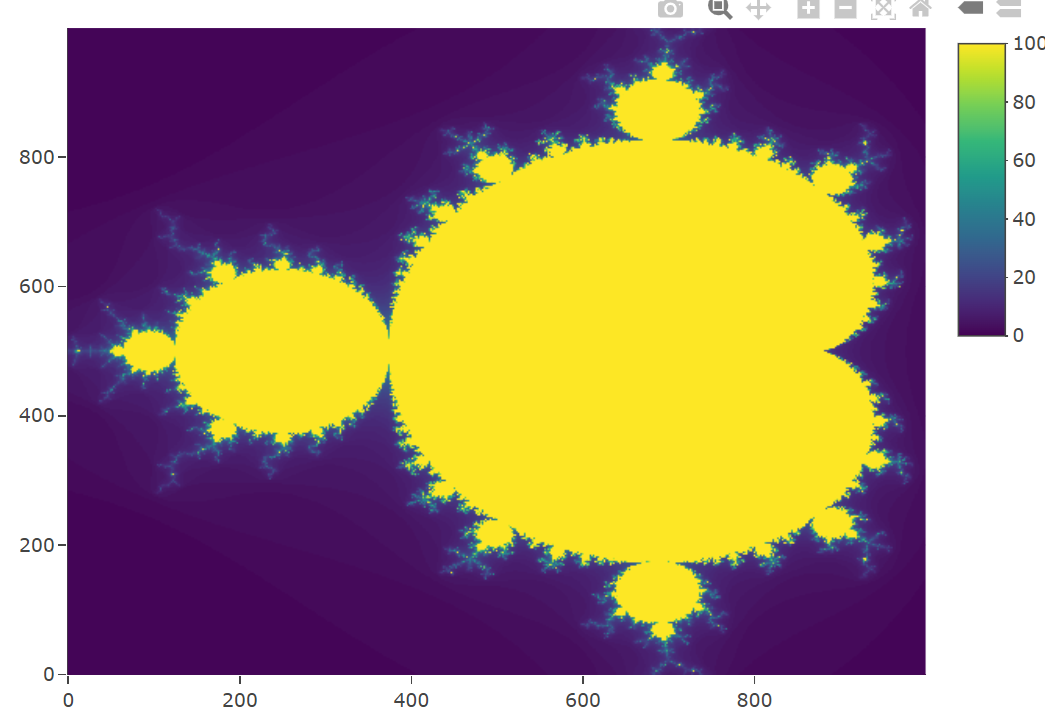
\includegraphics[width=140pt]{images/mandelbrot1.png}		
			
		\end{center} 
\end{frame}
	
\begin{frame}[fragile]{Inner algorithm in {\tt R}}
For any point $c=a+ib\in\mathbb{C}$ we check, if it is in the Mandelbrot set by the following procedure:
\footnotesize 
\begin{verbatim}
mandelbrot <- function(c, max_iter = 100) {
  z <- c
  for (i in 1:max_iter-1) {
    z <- z ^ 2 + c
    if (abs(z) > 2) {
      return(i)
    }
  }
  return(max_iter)
}
\end{verbatim}

\end{frame}
	

\begin{frame}[fragile]{Inner algorithm in C++}
	C++ code for the inner algorithm using {\tt Rcpp}:
	\scriptsize 
\begin{verbatim}
Rcpp::cppFunction(
"
int Mandel(double real, double im, int max_iter = 100)
{
  std::complex<double> c(real, im);
  std::complex<double> z = c;
  for (int i=0; i< max_iter; i++){
    z = z * z + c;
    if (std::abs(z) > 2) {
      return i;
    }
  }
  return max_iter;
}
"
)
\end{verbatim}
\end{frame}

\begin{frame}{Outer (meta) algorithm}

\begin{itemize}
	\item[1.] Input: $A$ - discrete rectangular grid of complex points between $c_{\min}=-1.5-i$ and $c_{\max}=0.5+i$ with resolution 1000 in each dimension.
	\item[2.] For every point $c\in A$ check, if it is in the Mandelbrot set by the inner algorithm.
	\item[3.] Visualise the results.
\end{itemize}	
\end{frame}




\begin{frame}{Three implementations}
	
	\begin{itemize}
		\item[1.] The outer and the inner algorithm written in {\tt R}
		\item[2.] The outer in {\tt R }and the inner algorithm in {\tt C++}
		\item[3.] The outer and the inner algorithm written in {\tt C++}
	\end{itemize}	\pp 
	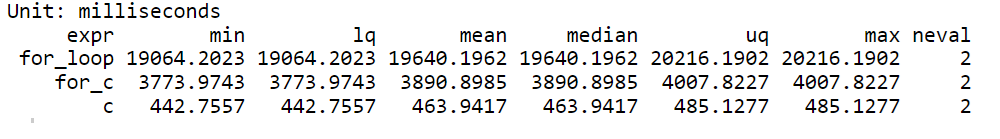
\includegraphics[width=250pt]{images/mandelbrot}
\end{frame}



\end{document}

